\documentclass[msc,deptreport,cs]{infthesis} % Do not change except to add your degree (see above).

%% Imports poached from frankly
%% STILL can't find what makes \figrule work
\usepackage{natbib}
\usepackage{mathpartir}
\usepackage{amsmath}
\usepackage{amsfonts}
\usepackage{thmtools,thm-restate}
\usepackage{comment}
\usepackage{flushend}
\usepackage{listings}
\usepackage{lstlinebgrd}
%% \usepackage{beramono}

%% \lstdefinestyle{mystyle}{
%%     %% backgroundcolor=\color{backcolour},
%%     %% commentstyle=\color{codegreen},
%%     %% keywordstyle=\color{magenta},
%%     %% numberstyle=\tiny\color{codegray},
%%     %% stringstyle=\color{codepurple},
%%     breakatwhitespace=false,
%%     breaklines=true,
%%     captionpos=b,
%%     keepspaces=true,
%%     %% numbers=left,
%%     %% numbersep=5pt,
%%     showspaces=false,
%%     showstringspaces=false,
%%     showtabs=false,
%%     tabsize=2,
%%     %% basicstyle=\small\ttfamily
%%     basicstyle=\ttfamily\footnotesize,
%%     %% breaklines=true
%% }

%% \lstset{style=mystyle}

%% \lstset{escapeinside={<@}{@>}}

\lstset{
  %% basicstyle=\small\ttfamily\bfseries,
  basicstyle=\footnotesize\ttfamily\bfseries,
  %% basicstyle=\footnotesize\ttfamily,
  %% basicstyle=\small\ttfamily,
  breaklines=true,
  % For having lighter-coloured text inside listings
  % https://tex.stackexchange.com/questions/144448/color-a-text-line-in-a-code-lstlisting
  escapeinside={<@}{@>}
}


\usepackage{stmaryrd}
\usepackage{natbib}
\usepackage{xspace}
%% \usepackage[pdftex,
%%             pdfauthor={Sam Lindley, Conor McBride, and Craig McLauglin},
%%             pdftitle={Doo bee doo bee doo}]{hyperref}
%\hypersetup{colorlinks=true,citecolor=blue,linkcolor=blue}
%% \hypersetup{colorlinks=true,allcolors=black}
\usepackage[usenames,dvipsnames]{xcolor}
\usepackage{url}

% get rid of hypertext link on \citeauthor
\usepackage{etoolbox}

\usepackage{amssymb}

\usepackage{mathtools} % allows flush-left align environments and paired
                       % delimiters.
                       %
\usepackage{hyperref}
\hypersetup{
    colorlinks,
    citecolor=black,
    filecolor=black,
    linkcolor=black,
    urlcolor=black
}

% Theorem environments
\newtheorem{theorem}{Theorem}
\newtheorem{proposition}[theorem]{Proposition}
\newtheorem{definition}[theorem]{Definition}
\newtheorem{prop}[theorem]{Proposition}
\newtheorem{lemma}[theorem]{Lemma}
\newtheorem{corollary}[theorem]{Corollary}


%% abstract for inline code
\newcommand{\code}[1]{\lstinline{#1}}
\newcommand{\codem}[1]{\lstinline[mathescape]{#1}}


\newcommand{\highlight}[1]{%
  \colorbox{red!20}{$\displaystyle#1$}}

\newcommand{\texthighlight}[1]{%
  \colorbox{red!20}{#1}}

\newcommand{\highlightout}[1]{%
  \colorbox{black!20}{$\displaystyle#1$}}

\newcommand{\greytext}[1]{\textcolor{black!40}{#1}}

\newcommand\aeff{{\AE}ff\xspace}

\newcommand\nondetfrank{$\mathbb{F}_{\cal{ND}}$}
\newcommand\countingfrank{$\mathbb{F}_{\cal{C}}$}

%%%%%%%%%%%%%%%%%%%%%%%%%%%%%%%%%%%%%%%%%%%%%%%%%
%% Start of inference rules typesetting business
%%%%%%%%%%%%%%%%%%%%%%%%%%%%%%%%%%%%%%%%%%%%%%%%%
%%%%%%%%%%%%%%%%%%%%%%%%%%%%%%%%%%%%%%%%%%%%%%%%%


\newcommand{\counter}{{\color{blue}c_y}}
\newcommand{\justc}[1]{{\color{blue} c({#1})}}
\newcommand{\yieldc}{{\color{blue}{\textsf{yield}}}}
\newcommand{\plusc}{{\color{blue} +_c}}
\newcommand{\threshc}{{\color{blue} t_y}}

\newcommand\yield{\textsf{yield}\xspace}
\newcommand\Yield{\textsf{Yield}\xspace}
\newcommand\allows{\textsf{allows}\xspace}


\DeclarePairedDelimiter{\ceil}{\lceil}{\rceil}

\newcommand{\todo}[1]
           {{\par\noindent\small\color{RoyalPurple}
  \framebox{\parbox{\dimexpr\linewidth-2\fboxsep-2\fboxrule}
    {\textbf{TODO:} #1}}}}

\newcommand{\interrupt}[1]{!(#1)}

\newcommand{\fighead}{\textbf}

\newcommand{\lameff}{$\lambda_{\text{eff}}$\xspace}
\newcommand{\lameffrow}{$\lambda_{\text{eff}}^\rho$\xspace}
\newcommand{\feff}{$F_\textrm{eff}$\xspace}
\newcommand{\impeff}{Implicit \lameff}
\newcommand\Frank{\emph{Frank}\xspace}

\newcommand\Cse{\textbf{Case}}

\newcommand{\set}[1]{\{#1\}}
\newcommand{\many}{\overline}
\newcommand{\opt}[1]{#1^?}
\newcommand{\medvert}{\mid}

\newcommand{\sem}[1]{\llbracket{#1}\rrbracket}
\newcommand{\seml}{\left\llbracket}
\newcommand{\semr}{\right\rrbracket}

\newcommand{\mdo}{~\textbf{do}~}
\newcommand{\seq}{~\textbf{;}~}
\newcommand{\assn}[2]{{#1}~\leftarrow~{#2}}
\newcommand{\func}[2]{\text{#1}~{#2}}

\newcommand{\deno}[1]{\sem{#1}\rho}
\newcommand{\denoex}[2]{\sem{#1}#2}
\newcommand{\pc}[1]{\llparenthesis{#1}\rrparenthesis}

\newcommand{\TyVar}{\mathit{Var}}
\newcommand{\dom}{\mathit{dom}}
%\newcommand{\sub}{\subseteq}
\newcommand{\Star}{{\Large$\star$}}

\newcommand{\reducesto}{\longrightarrow}

\newcommand\ba{\begin{array}}
\newcommand\ea{\end{array}}

\newcommand{\bl}{\ba[t]{@{}l@{}}}
\newcommand{\el}{\ea}

\newcommand{\bstack}{\begin{array}[t]{@{}l@{}}}
\newcommand{\estack}{\end{array}}

\newenvironment{equations}{\[\ba{@{}r@{~}c@{~}l@{}}}{\ea\]\ignorespacesafterend}
\newenvironment{eqs}{\ba{@{}r@{~}c@{~}l@{}}}{\ea}

\newenvironment{clauses}{\ba{@{}l@{~}c@{~}l@{}}}{\ea}

\newenvironment{syn}{\ba{@{}l@{~}r@{~}c@{~}l@{}}}{\ea}

\newenvironment{syntax}{\[\ba{@{}l@{~}r@{~}c@{~}l@{}}}{\ea\]\ignorespacesafterend}

\newcommand{\judgeword}[1]{~\mathbf{#1}~}

%\renewcommand{\sig}{\Sigma}
%\renewcommand{\sigs}{\Sigma s}
\newcommand{\sigentails}[1]{\mathbin{[{\text{\scriptsize ${#1}$}}]\hspace{-0.4ex}\text{-\!-}}\,}

%% \newcommand{\sigmodels}[1]{\mathbin{[{\text{\scriptsize ${#1}$}}]\!\mathord{=}}\,}
% \newcommand{\sigentails}[1]{\vdash_{#1}}

\newcommand{\val}[3]  {#1 \vdash {#2} : {#3}}

\newcommand{\rt}[1]{\langle{#1}\rangle}   % returner type

\newcommand{\valg}{\val{\Gamma}}

%% \newcommand{\is}[4]  {#1 \sigentails{#2} {#3} \judgeword{is} {#4}}
%% \newcommand{\isgs}{\is{\Gamma}{\sigs}}

%% \newcommand{\cdoes}[4]{#1 \sigentails{#2} {#3} \judgeword{has} {#4}
%% \newcommand{\cdoesgs}{\cdoes{\Gamma}{\sigs}}


%% some options for rendering bidirectional typing judgements

%% \newcommand{\inferbase}[4]{#2 \mathbin{#1} {#3} \in {#4}}
%% \newcommand{\checkbase}[4]{#2 \mathbin{#1} {#3} \ni {#4}}
%% \newcommand{\patbase}[4]{{#3} \mathbin{:} {#2} \mathbin{#1} {#4}}

\newcommand{\kindcheckbase}[3]{#2 \mathbin{#1} #3} % For well-kindedness of types
\newcommand{\inferbase}[5]{#1; #3 \mathbin{#2} {#4} \Rightarrow {#5}}
\newcommand{\checkbase}[5]{#1; #3 \mathbin{#2} #5 \mathbin{:} #4}
\newcommand{\patbase}[5]{{#1} \vdash {#4} \mathbin{:} {#3} \mathbin{#2} {#5}}
\newcommand{\bindbase}[4]{{#3} \mathbin{:} {#2} \mathbin{#1} {#4}}

%% \newcommand{\inferbase}[4]{#2 \mathbin{#1} {#3} \Rightarrow {#4}}
%% \newcommand{\checkbase}[4]{#2 \mathbin{#1} {#4} \Leftarrow {#3}}
%% \newcommand{\patbase}[4]{{#3} \mathbin{:} {#2} \mathbin{#1} {#4}}

%% \newcommand{\inferbase}[4]{#2 \mathbin{#1} {#3} \uparrow {#4}}
%% \newcommand{\checkbase}[4]{#2 \mathbin{#1} {#4} \downarrow {#3}}
%% \newcommand{\patbase}[4]{{#3} \mathbin{:} {#2} \mathbin{#1} {#4}}

%% \newcommand{\inferbase}[4]{#2 \mathbin{#1} {#3} \judgeword{infers} {#4}}
%% \newcommand{\checkbase}[4]{#2 \mathbin{#1} {#3} \judgeword{checks} {#4}}
%% \newcommand{\patbase}[4]{{#2} \judgeword{matches} {#3} \mathbin{#1} #4}

\newcommand{\makes}[5]{\inferbase{#1}{\sigentails{#3}}{#2}{#4}{#5}}
\newcommand{\has}[5]{\checkbase{#1}{\sigentails{#3}}{#2}{#4}{#5}}
\newcommand{\does}[4]{\checkbase{#1}{\vdash}{#2}{#3}{#4}}
\newcommand{\can}[4]{\makes{\kenv}{#1}{#2}{#3}{#4}}

\newcommand{\effs}[2]{{#1} \judgeword{does} {#2}}


% redefinitions for cbv type system
\newcommand{\kindchecks}[2]{\kindcheckbase{\vdash}{#1}{#2}} % Checks that a type is well-kinded
\newcommand{\infers}{\makes}
\newcommand{\checks}{\has}
\newcommand{\checksdef}{\does}
\newcommand{\matchesc}{\matches}
\newcommand{\matchesck}{\matchesc{\kenv}}

\newcommand{\infersk}{\makes{\kenv}}
\newcommand{\checksk}{\has{\kenv}}
\newcommand{\checksdefk}{\does{\kenv}}

\newcommand{\kindchecksk}{\kindchecks{\kenv}} % Checks that a type is well-kinded
\newcommand{\inferskgs}{\makes{\kenv}{\Gamma}{\sigs}}
\newcommand{\checkskgs}{\has{\kenv}{\Gamma}{\sigs}}
\newcommand{\checksdefkg}{\does{\kenv}{\Gamma}}


\newcommand{\adj}{\Delta}
\newcommand{\adapt}{\Theta}
\newcommand{\ext}{\Xi}
\newcommand{\sigs}{\Sigma}
\newcommand{\sig}{I}

\newcommand{\seed}{\sigma}

\newcommand{\effbox}[1]{[#1]}

\newcommand{\key}[1]{\mathbf{#1}} % keyword
\newcommand{\var}{\mathit}        % local variable or meta variable
\newcommand{\defaultvarname}[0]{x}

\newcommand{\op}{\mathsf}  % operator (command or computation)
\newcommand{\con}{\mathsf} % constructor (type or data)
\newcommand{\inter}{\mathsf} % interface
\newcommand{\str}[1]{\textrm{``#1''}} % string literal


\newcommand{\handleSymbol}{\rightarrow}
\newcommand{\handle}[2]{{#1} \handleSymbol {#2}}

\newcommand{\thunk}[1]{\{{#1}\}}

\newcommand{\force}[1]{{#1}!}

\newcommand{\emptylist}{[]}
\newcommand{\cons}{\mathbin{::}}
\newcommand{\concat}{\,\texttt{++}\,} %mathbin{+\!+}}
%\newcommand{\snoc}{\mathbin{:<}}
\newcommand{\snoc}{\ }


\newcommand{\NN}{\mathbb{N}}

\newcommand\slab[1]{(\textrm{#1})}

\newcommand{\ev}{E}
\newcommand{\evd}{\varepsilon}

\newcommand{\effin}[1]{\langle {#1} \rangle}
\newcommand{\effout}[1]{[{#1}]}

\newcommand{\nowt}{\emptyset}
\newcommand{\id}{\iota}
\newcommand{\pid}{\var{s}} % Pattern identity variable

\newcommand{\EC}{\mathcal{E}}
\newcommand{\EF}{\mathcal{F}}
\newcommand{\PC}{\mathcal{P}} % Syntactic phrase class for af operation
\newcommand{\venv}{\theta}

\newcommand{\freeze}{\ceil}

\newcommand{\uc}{\mathord{\downarrow}}
\newcommand{\cu}{\mathord{\uparrow}}

\newcommand{\redtou}{\leadsto_{\mathrm{u}}}
\newcommand{\redtoc}{\leadsto_{\mathrm{c}}}
\newcommand{\stepsto}{\longrightarrow}

\newcommand{\stepstou}{\longrightarrow_{\mathrm{u}}}
\newcommand{\stepstoc}{\longrightarrow_{\mathrm{c}}}

\newcommand{\sigat}{\mathbin{@}}

\newcommand{\meta}{\mathsf}
\newcommand{\level}{\meta{level}}
\newcommand{\af}{\meta{af}}
\newcommand{\handles}{~\meta{handles}~}

\newcommand{\poised}{~\meta{poisedfor}~}
\newcommand{\insts}{\meta{inst}}
\newcommand{\remap}{\meta{remap}}

\newcommand{\sigyields}[1]
           {\mathbin{\text{-\!-\!}[{\text{\scriptsize ${#1}$}}]\,}}

\newcommand{\matches}[5]{\patbase{#1}{\sigyields{#4}}{#2}{#3}{#5}}
\newcommand{\matchesv}[4]{\patbase{#1}{\dashv}{#2}{#3}{#4}}
\newcommand{\matchesvk}{\matchesv{\kenv}}

\newcommand{\bindsv}[4]{\bindbase{\dashv}{#2 \leftarrow #3}{#1}{#4}}
\newcommand{\bindsc}[5]{\bindbase{\sigyields{#4}}{#2 \leftarrow #3}{#1}{#5}}

\newcommand{\letin}[4][\defaultvarname]
           {\key{let}\;{#1}:{#2}={#3}\;\key{in}\;{#4}}
\newcommand{\letxin}[3][\defaultvarname]
           {\key{let}\;{#1}={#2}\;\key{in}\;{#3}}
\newcommand{\letrec}[4][f]{\key{letrec}~\many{{#1}:{#2} = {#3}}~\key{in}~{#4}}
\newcommand{\letrecU}[3][f]{\key{letrec}~\many{{#1} = {#2}}~\key{in}~{#3}}
\newcommand{\Gt}{\theta} % Substitution meta variable
\newcommand{\submap}[2]{{{#1}\vDash{#2}}}
\newcommand{\sub}[4]{#1 \vdash {{#2}:\submap{{#3}}{{#4}}}}
\newcommand{\subk}{\sub{\kenv}}
\newcommand{\subext}[2]{{{#1}{#2}}}
\newcommand{\subst}[3][\defaultvarname]{{#2}[{#3}/{#1}]}

% Frank letrec substitution
\newcommand{\recsub}[5][f]
      {[\many{\cu (\thunk{\many{\many{#2}\mapsto\letrec[{#1}]{#5}{#3}{#4}}}
            : {#5})/{#1}}]}


%%%% START inference rule system for action of adjustment on ability %%%%
\newcommand{\semi}{;}
\newcommand{\kenv}{\Phi}  % kind environment
\newcommand{\kenva}{\Psi} % another kind environment
%% \newcommand{\kenv}{\mathcal{T}} % kind environment
\newcommand{\ienv}{\Omega} % Instance environment
\newcommand{\adjact}[3]{{#1}\vdash{#2}\dashv{#3}}
\newcommand{\adpcom}[5]{{{#1}\vdash{#2}({#3} \to {#4})\dashv{#5}}}
\newcommand{\itrbnd}[5]{{{#1}\vdash{#2}:{#3}\dashv{#4}\semi{#5}}}
% \newcommand{\wf}[2]{{{#1}\vdash{#2}}}
\newcommand{\itrinst}[4]{{{#1}\vdash{#2}:{#3}\dashv{#4}}}

%%% END inference rule system for action of adjustment on ability %%%%%

% Untyped machine letrec substitution
\newcommand{\recsubst}[5]
 {{#1}[\many{(\thunk{\many{\many{#2} \mapsto \letrecU{#3}{#4}}}:{#5})/f}]}

%% Abstract machine commands
% Typing
\newcommand{\HAbs}[2]{{{#1}\to{#2}}}

\newcommand{\fail}{\textbf{fail}}

%% Translation function: Frank Terms to Untyped A-Normal Form
\newcommand{\UANF}[1]{{\llbracket{{#1}}\rrbracket}}

% Terms
\newcommand{\mtrns}[3][]{{#2} & \Rightarrow^{#1} & {#3}} % For array env
\newcommand{\mtrnsR}[3][]{{#2}\Rightarrow^{#1}{#3}}

\newcommand{\confg}[2]{{\langle{{#1}},{{#2}}\rangle}}
\newcommand{\term}[3]
           {{\langle{{#1}},{{#2}}\rangle\downarrow{#3}}}

\newcommand{\admin}[2]{{\langle{{#1}}\mid{{#2}}\rangle}}
\newcommand{\mat}[3]
           {{\langle{{#1}}\mid{{#2}}\mid{{#3}}\rangle}}
\newcommand{\matc}[5]
        {{\langle{{#1}}\mid{{#2}}\mid{{#3}}\mid{{#4}}\mid{{#5}}\rangle}}

\newcommand{\msub}[3][\defaultvarname]{{#2}[{#1}\mapsto{#3}]}

\newcommand{\FHan}[4][\many{\effin{\adj}}]{{({#2}:{#1},{#3}\mid{#4})}}
\newcommand{\FSeq}[2][\defaultvarname]
           {{({#1}.{#2})}}
\newcommand{\SCons}[2]{{{#1}\circ{#2}}}


\newcommand{\HSHan}[5][C]{{{#2}\circ({#3},{#1},{#4}\mid{#5})}}
\newcommand{\HSSeq}[4][\defaultvarname]
           {{#2}\circ({#1}:{#3}.{#4})}
\newcommand{\HSCons}[2]{{{#1}\circ{#2}}}
\newcommand{\NF}[2]{{{#1}~\star~{#2}}}

\newcommand{\evalto}{\Longrightarrow}


\newcommand{\para}[1]{\paragraph{#1.}}

\newcommand{\gor}{\mid}
\newcommand{\pipe}{\texttt{|}}


%%%%%%%%%%%%%%%%%%%%%%%%%%%%%%%%%%%%%%%%%%%%%%%%%
%% End of inference rules typesetting business
%%%%%%%%%%%%%%%%%%%%%%%%%%%%%%%%%%%%%%%%%%%%%%%%%






%%%%%%%%%%%%%%%%%%%%%%%%%%%%%%%%%%%%%%%%
%% Start of main text
%%%%%%%%%%%%%%%%%%%%%%%%%%%%%%%%%%%%%%%%

\begin{document}
\begin{preliminary}

\title{Asynchronous Effect Handling 2}

\author{Leo Poulson}

\abstract{
  Features for asynchronous programming are commonplace in the programming
  languages of today, allowing programmers to issue tasks to run on other
  threads and wait for the results to come back later. This is particularly
  useful for programs like web programs, etc...

  In this thesis we show how asynchronous programming can be very easily
  accomodated in a language with existing support for effect handlers. We show
  how, with a small change to the language implementation, truly asynchronous
  programming with pre-emptive concurrency is achieved.
}

\maketitle

\section*{Acknowledgements}
thanks!

\tableofcontents

\end{preliminary}

\chapter{Introduction}

Effects, such as state and nondeterminism, are pervasive when programming; for a
program to do anything beyond compute a pure mathematical function, it must
interact with the outside world, be this to read from a file, make some random
choice, or run concurrently with another program. Algebraic effects and their
handlers are a novel way to encapsulate, reason about and specify computational
effects in programming languages. For instance, a program that reads from and
writes to some local state can utilise the \textsf{State} effect, which supports
two \emph{operations}; \textsf{get} and \textsf{put}. A handler for the
\textsf{State} effect gives a meaning to these abstract operations.

Programming with effects is increasingly popular, references, ...

Traditional effect handling is \emph{synchronous}; when an effectful operation
is invoked, the rest of the computation pauses whilst the effect handler
performs the requisite computation and then resumes the original caller.
\todo{Do we need to speak about how the continuation of the caller gets 'offered
  up'?}
%
For many effects, this blocking behaviour is not a problem; the handler usually
returns quickly, and the user does not notice anything. Of course, not every
possible computational effect behaves like this. Consider an effect involving a
query to a remote database. We might not want to block the rest of the
computation whilst we perform this, as the query might take a long time; this
case is even stronger if we do not immediately want the data. To support this
kind of behaviour, we need to be able to invoke and handle effects in an
asynchronous, non-blocking manner.

\texthighlight{In this project we investigate the implementation and
  applications of asynchronous effects}. Our lens for this is the language
Frank~(\cite{convent2020doo}), a functional programming designed with effect
handlers at its core. We follow the design
of~\aeff~(\cite{ahman2020asynchronous}), a small programming language designed
around asynchronous effects but supporting little else. We show how, with a
small change to the semantics of Frank, we can recreate the asynchronous effect
handling behaviour of~\aeff.

\todo{Talk about extra examples...}

%% The changes made to Frank are straightforward to recreate, and whilst the Frank
%% library for programming with asynchronous effects enjoys some specific

Frank is a well-suited language for an asynchronous effects library, especially
because of the fine-grained control over suspended computations, making it very
easy to treat code as data. Despite this, our approach does not use any specific
Frank features; furthermore, the changes made to the semantics of Frank are
easily recreateable. It is our hope that these methods could be recreated in
another language equipped with first-class effect handlers. Effect handlers have
already proven to make complicated control flow easy to implement
(\textbf{refs}), and our work further cements this viewpoint.

\section{Related Work}

TFP, aeff, etc
\section{Contributions}

\paragraph*{Asynchronous Effects Library} We present a library for programming
with asynchronous effects in the style of \aeff, built in Frank. We show how a
complex system can be expressed concisely and elegantly when programming in a
language with effect handlers, further cementing the case for effects as a
foundation for concurrent programming. \todo{Rewrite the end of this; slightly
  messy}.

\paragraph*{Pre-emptive Concurrency} We show how, by making a small change to
the operational semantics of Frank, we achieve pre-emptive concurrency; that is,
the suspension of running threads \emph{without} co-operation. It is our hope
that this change is simple enough to be transferrable to other languages.

\paragraph*{Examples} We also deliver a set of examples of the uses of
asynchronous effects, and show how they have benefits to other models.

\section{Structure}

In Chapter~\ref{chap:programming-in-frank} we give an introduction to
programming with effects in Frank. We skip over some unneeded parts, such as
adaptors, in the interests of time.

In Chapter~\ref{chap:formalisation} we give the formalisation of Frank. Again,
we skip over extraneous details which can be seen in past work
(\cite{convent2020doo}), opting to only describe the parts needed to understand
the changes to the semantics for the following chapter.

In Chapter~\ref{chap:preemptive-concurrency} we show how by making a small
change to the semantics of Frank we yield pre-emptible threads; that is, we can
interrupt a function in the same 'co-operative' style but without co-operation

\todo{Fix above}

In Chapter~\ref{chap:implementation} we describe the implementation of our
asynchronous effect handling library in Frank. In Chapter~\ref{chap:examples} we
give examples of the new programs that become easily expressible when combined
with the changes made in Chapter~\ref{chap:preemptive-concurrency}.

In Chapter~\ref{chap:conclusion} we conclude.






\chapter{Programming in Frank}
\label{chap:programming-in-frank}

Frank is a functional programming language, designed with the use of algebraic
effects at its heart. As such, Frank has an effect type system used to track
which effects a computation may use.

Frank offers very fine-grained control over computations. It clearly
distinguishes between computation and value, and offers \emph{multihandlers} to
carefully control when computations are evaluated. This combined with effect
handling provides a very rich foundation for expressing complex control
structures.

In this chapter we introduce Frank, and show why it is so well-suited to our
task. We assume some familiarity with typed functional programming, and skip
over some common features of Frank --- algebraic data types, pattern matching,
etc. --- so we can spend more time with the novel, interesting parts.

\section{Types, Values and Operators}

Frank types are distinguished between \emph{effect types} and \emph{value
  types}. Value types are the standard notion of type; effect types are
used to describe where certain effects can be performed and handled. Value types are further divided into traditional data types, such a \code{Bool},
\code{List X}, and \emph{computation types}.

A computation type
%
\lstinline[mathescape]!X$_1$ -> ... -> X$_m$ -> [I$_1$, ..., I$_n$]Y!
%
%% This type expresses that the operator can handle some effect in the first
%% argument and then performs some other effects as a result, returning a value of
%% type \code{Y}.
expresses that we take $m$ arguments and return a value of type \code{Y}. The
return type expresses the \emph{ability} the computation needs access to, being
a list of $n$ \emph{interface} instances. An interface is a collection of
\emph{commands} which are offered to the computation.

%% Frank then specialises effect handling to traditional function application; a
%% function is the special case of an operator that handles no arguments. We see
%% that a function type \code{\{X -> Y -> Z\}} is just a special case of the
%% general operator type where no effects are handled or performed. Throughout this
%% thesis, we call

Thunks are then the special case of an $n$-ary function that takes 0 arguments.
We can evaluate them --- performing the suspended computation --- with the 0-ary
sequence of arguments, denoted \code{!}. Computations are suspended by wrapping
them in braces.

This gives us fine-grained control over when we want to evaluate computations.
For instance, we might want the sequential composition operator \code{snd} (also
commonly known as the semicolon operator);

\begin{lstlisting}
  snd : {X -> Y -> Y}
  snd x y = y
\end{lstlisting}

Frank is a left-to-right call-by-value language; arguments to functions are
evaluated from left-to-right, until they become a value. In the case of
\code{snd}, \code{x} is first evaluated, then \code{y}, which is finally
returned. Compare this to \code{if};

\begin{lstlisting}
if : {Bool -> {X} -> {X} -> X}
if true  yes no = yes!
if false yes no = no!
\end{lstlisting}

\noindent The branches are given as thunks, where a single thunk is evaluated
depending on the condition. If we did not take this approach both cases would be
evaluated, which is clearly not the intended semantics of \code{if}. Frank's
distinction between computation and value make controlling evaluation simple and
pleasing.

%% \todo{Example --- maybe fire missiles one?}

\section{Effects and Effect Handling}
\label{sec:effects}

\paragraph*{Interfaces and Operations}

Frank encapsulates effects through \emph{interfaces}, which offer
\emph{commands}. For instance, the \code{State} effect (interface) offers two
operations (commands), \code{get} and \code{put}. In Frank, this translates to

\begin{lstlisting}
  interface State X = get : X
                    | put : X -> Unit

  interface RandInt = random : Int
\end{lstlisting}

The type signatures of the operations mean that \code{get} is a 0-ary operation
which is \emph{resumed} with a value of type \code{X}, and \code{put} takes a
value of type \code{X} and is resumed with \code{unit}. Computations get access
to an interface's commands by including them in the \emph{ability} of the
program. Commands are invoked just as normal functions;

\begin{lstlisting}
  xplusplus : {[State Int] Unit}
  xplusplus! = put (get! + 1)
\end{lstlisting}

\noindent This familiar program increments the integer in the state by 1.

\paragraph*{Handling Operations}

%% Traditional functions in Frank are a specialisation of Frank's handlers; that is
%% to say, functions are handlers that handle no effects. A handler for an
%% interface pattern matches \emph{on the operations} that are invoked, as well as
%% on the \emph{values} that the computation can return. Furthermore, the handler
%% gets access to the \emph{continuation} of the calling function as a first-class
%% value. Consider the handler for \code{State};

A handler for a specific interface can also pattern match on the
\code{operations} that are performed, and not just the values that can be
returned. As an example, consider the canonical handler for the \code{State S}
interface.

\begin{lstlisting}
  runState : {<State S> X -> S -> X}
  runState <get -> k>   s = runState (k s) s
  runState <put s -> k> _ = runState (k unit) s
  runState x            _ = x
\end{lstlisting}

%% \noindent The type of \code{runState} expresses that the first argument is a
%% computation that can perform \code{State S} effects and will eventually return a
%% value of type \code{X}, whilst the second argument is a value of type \code{S}.

\noindent Observe that the type of \code{runState} contains \code{<State S>},
called an \emph{adjustment}. This expresses that the first argument can perform
commands in the \code{State S} interface, and that \code{runState} must handle
these commands if they occur.

\subparagraph*{Computation Patterns}
The second and third lines specify how we handle \code{get} and \code{put}
commands. Observe that we use a new type of pattern, called a \emph{computation
  pattern}; these are made up of a command and some arguments (which are also
values), plus the continuation of the calling code. The types of arguments and
the continuation are determined by the interface declaration and the type of the
handler; for instance, in \code{<get -> k>} the type of \code{k} is \code{\{S ->
  [State S] X\}}. The continuation can then perform more \code{State S} effects.
This differs to some other implementations of effect handling languages
\todo{Add references} where the handlers are \emph{deep}, meaning the
continuation has been re-handled by the same handler automatically.

What happens when we run \code{runState xplusplus! 0}? When a computation is
invoked, it is performed until it results in either a \emph{value} or a
\emph{command}. Thus, \code{runState} will be paused until \code{xplusplus!}
reduces; \code{runState} is resumed when \code{xplusplus} is in one of these two
forms.

\code{xplusplus} instantly invokes \code{get!}. At this point, control is given
to the handler \code{runState}; both in the sense that \code{runState} is now
being executed by the interpreter, and that \code{runState} has control over the
\emph{continuation} of \code{xplusplus}, which is a function of type \code{Int
  -> [State Int] Unit}. We see that \code{runState} chooses to resume this
continuation with the value of the state at that time.

\paragraph*{Effect Forwarding}

Effects that are not handled by a particular handler are left to be forwarded up
to the next highest one. For instance, we might want to write a random number to
the state;

\begin{lstlisting}
  xplusrand : {[State Int, RandomInt] Unit}
  xplusrand! = put (random!)
\end{lstlisting}

\noindent We then have to handle both the \code{State Int} and \code{Random}
effect in this computation. Of course, we could just define one handler for both
effects; however in the interests of \emph{modularity} we want to define two
different handlers for each effect and \emph{compose} them. We can reuse the
same \code{runState} handler from before, and define a new handler for
\code{RandomInt};

\begin{lstlisting}
  runRand : {Int -> <RandomInt> X -> X}
  runRand seed <random -> k> = runRand (mod (seed + 7) 10) (k seed)
  runRand _ x = x
\end{lstlisting}

\noindent And compose them in the comfortable manner, by writing \code{runRand
  (runState xplusrand!)}.

\todo{Maybe show example of how the order of composition can change the ending
  semantics --- a la state + aborting}

\paragraph*{Top-Level Effects}
Some effects need to be handled outside of pure Frank, as Frank is not
expressive or capable enough on its own. Examples are console I/O, web requests,
and ML-style state cells. These effects will pass through the whole stack of
handlers up to the top-level, at which point they are handled by the
interpreter.






\paragraph*{Implicit Effect Polymorphism}

Consider the type of the well-known function \code{map} in Frank;

\begin{lstlisting}
  map : {{X -> Y} -> List X -> List Y}
  map f [] = []
  map f (x :: xs) = (f x) :: (map f xs)
\end{lstlisting}

\noindent One might expect that the program \code{map \{_ -> random!\} [1, 2, 3]}
would give a type error; we are mapping a function of type \code{\{Int ->
  [RandomInt] Int\}}, which does not match the argument type \code{\{X -> Y\}}.
However, Frank uses a shorthand for \emph{implicit effect variables}. The
desugared type of \code{map} is actually

\begin{lstlisting}[mathescape]
  map : {{X -> [$\epsilon$|] Y} -> List X -> [$\epsilon$|] List Y}
\end{lstlisting}

\noindent This type expresses that whatever the ability is of \code{map f xs} will be
offered to the element-wise operator \code{f}. As such, the following
typechecks;

\begin{lstlisting}
  writeRand : {List Int -> [RandomInt] List Int}
  writeRand xs = map {_ -> random!} xs
\end{lstlisting}

\todo{Talk about deliberately stopping this}

\todo{Talk about what the bar means. }

A similar thing happens in interface declarations. We might define the
\code{Choose} effect, which non-deterministically asks for one of two
computations to be picked for it to continue with;

\begin{lstlisting}
  interface Choose X =
      choose : {[Choose X] X} -> {[Choose X] X} -> X
\end{lstlisting}

\noindent This definition desugars to

\begin{lstlisting}[mathescape]
  interface Choose X [$\epsilon$] =
      choose : {[$\epsilon$| Choose X] X} -> {[$\epsilon$| Choose X] X} -> X
\end{lstlisting}

\noindent Once again, an implicit effect variable is inserted in every ability
available.




\paragraph*{Synchronicity and Conversations}
Observe how the interaction between the effect invoking function and the handler
of this effect becomes like a conversation; the caller asks the handler for a
response to an operation, and the caller will then wait, blocking, for a
response. This can be characterised as \emph{synchronous} effect handling.

But what if we want to make a request for information, then do something else,
then pick up the result later when we need it? This is the canonical example of
asynchronous programming. It is not as simple as just invoking our e|.g.
\code{getRequest} effect; computation would block once this is invoked, meaning
we are stuck waiting for the request to return.

This asynchrony is exactly what we search for in this project.

%% Frank's realisation of effects is through \emph{interfaces} which offer
%% \emph{commands}. For instance, the \code{State} effect (interface) offers two
%% operations (commands), \code{get} and \code{put}. In Frank, this translates to

%% \begin{lstlisting}
%%   interface State X = get : X
%%                     | put : X -> Unit
%% \end{lstlisting}

%% The type signatures of the operations mean that \code{get!}, when handled, will
%% be a value of type \code{X}, whilst \code{put x} once handled will be a value of
%% type \code{Unit}.

%% \code{get} and \code{put} are given meaning by defining a \emph{handler} for the
%% \code{State} interface. Handlers in Frank are very simple things; they take as
%% argument a computation that can perform effects. The handlers then pattern match
%% \emph{on the operations} that are invoked, as well as on the \emph{values} that the
%% computation can return. What makes effects not just a special kind of value is
%% that they also offer the \emph{continuation} of the caller as a first-class
%% value.

%% Here we display the handler for \code{State};

%% \begin{lstlisting}
%%   runState : {<State X> Y -> X -> Y}
%%   runState <get -> k>   s = runState (k s) s
%%   runState <put s -> k> _ = runState (k unit) s
%%   runState y            _ = y
%% \end{lstlisting}

\paragraph*{Multihandlers}
\label{para:multihandlers}

Recall that in Frank pure functions are just the special case of handlers that
handle no effects. Naturally, this notion extends to the $n$-ary case; we can
handle multiple effects from different sources are once. Handlers which handle
multiple effects simultaneously are unsurprisingly called \emph{multihandlers}.
This lets us write functions such as \code{pipe} (example due to \cite{convent2020doo});

\begin{lstlisting}[numbers=left]
interface Send X = send : X -> Unit

interface Receive X = receive : X
 
pipe : {<Send X>Unit -> <Receive X>Y -> [Abort]Y}
pipe <send x -> s> <receive -> r> = pipe (s unit) (r x)
pipe <_> y = y
pipe unit <_> = abort!
\end{lstlisting}

Line 5 states that \code{pipe} will handle all instances of the \code{Send}
effect in the first argument, all instances of the \code{Receive} effect in the
second, and might perform \code{Abort} commands along the way. The matching
clauses are also new to the reader; line 6 implements the communication between
the two functions. We reinvoke \code{pipe}, passing the payload \code{x} of
\code{send} to the continuation of \code{r}. Lines 7 and 8 make use of the
\emph{catch-all} pattern, \code{<m>}. This will match the invocation of any
effect that is handled by that argument, or a value, binding this to \code{m}.
In line 7, the catchall pattern matches either a \code{send} command or a value;
in this case, the receiver has produced a value, so we can return that. In line
8 \code{<_>} matches either a value or a \code{receive}; but it must be a
\code{receive} command, as the value case would have been caught above. Hence we
have a broken pipe, so the \code{abort} command is invoked. This can then be
caught by another handler, which can implement a recovery strategy.

\todo{Is it worth changing the example to match request on the left earlier?}

\paragraph*{Polymorphic Commands}

As well as having polymorphic interfaces, such as \code{State X}, parametrised
by e|.g.~the data stored in the state, Frank supports polymorphic
\emph{commands}. These are commands which can be instantiated for any type. An
example is ML-style references, realised through the \code{RefState} interface;

\begin{lstlisting}
  interface RefState = new X   : X -> Ref X
                     | read X  : Ref X -> X
                     | write X : Ref X -> X -> Unit
\end{lstlisting}

\noindent For instance, \code{new X} can be instantiated by supplying a value as
an argument. A \code{Ref X} cell is then returned as answer.

\section{Cooperative Concurrency}
\label{sec:concurrency}

Frank is a single-threaded language. It is fortunate, then, that effect handlers
give us a malleable way to run multiple program-threads ``simultaneously'' \todo
{This is poorly written --- fix}.

This is because the invocation of an operation not only offers up the
operation's payload, but also the \emph{continuation} of the calling
computation. The handler for this operation is then free to do what it pleases
with the continuation. For many effects, such as \code{getState}, nothing
interesting happens to the continuation; in the case of \code{getState}, it is
resumed with the value in state. But these continuations are first-class; they
can resumed, sure, but also stored elsewhere or even thrown away. As such, by
handling \code{Yield} operations, we easily pause and switch between several
threads.

\subsection{Simple Scheduling}
\label{subsec:simple-scheduling}

We introduce some simple program threads and some scheduling multihandlers, to
demonstrate how subtly different handlers generate different scheduling
strategies.

\begin{lstlisting}
interface Yield = yield : Unit

words : {[Console, Yield] Unit}
words! = print "one "; yield!; print "two "; yield!; print "three "; yield!

numbers : {[Console, Yield] Unit}
numbers! = print "1 "; yield!; print "2 "; yield!; print "3 "; yield!
\end{lstlisting}

First note the simplicity of the \code{Yield} interface; we have one operation
supported, which looks very boring; the operation \code{yield!} will just return
unit --- of course, it is the way we \emph{handle} yield that is more
interesting.

\begin{lstlisting}
-- Runs all of the LHS first, then the RHS.
scheduleA : {<Yield> Unit -> <Yield> Unit -> Unit}
scheduleA <yield -> m> <n> = scheduleA (m unit) n!
scheduleA <m> <yield -> n> = scheduleA m! (n unit)
scheduleA _ _ = unit

-- Lets two yields synchronise, then handles both
scheduleB : {<Yield> Unit -> <Yield> Unit -> Unit}
scheduleB <yield -> m> <yield -> n> = scheduleB (m unit) (n unit)
scheduleB <yield -> m> <n> = scheduleB (m unit) n!
scheduleB <m> <yield -> n> = scheduleB m! (n unit)
scheduleB _ _ = unit
\end{lstlisting}

\todo{Can maybe delete the 2nd and 3rd matches of scheduleB to make the point
  more clear?}

We see two multihandlers above. Each take two \code{yield}ing threads and
schedule them, letting one run at a time. \code{scheduleA} runs the first thread
to completion, and only then runs the second one; the first time that the second
thread \code{yield}s it is \emph{blocked}, and can no longer execute. As such,
the output of \code{scheduleA words! numbers!} is \code{one 1 two three 2 3
  unit}.

\code{scheduleB} is fairer and more profound. We run \code{scheduleB words!
  number!} and receive \code{one 1 two 2 three 3 unit}; \code{scheduleB} is fair
and will ``match'' the yields together. We step through slowly. First
\code{words!} will print \code{one}, then it will \code{yield}. At this point
--- recalling that multihandlers pattern match left-to-right --- the second
thread, \code{numbers!}, is allowed to execute. In the meantime, \code{words!}
is stuck as \code{<yield -> m>}; it cannot evaluate any further, it is
\emph{blocked}. Whilst \code{words} is blocked \code{numbers!} prints \code{1}
and then \code{yield}s. Great; now the first case matches. Both threads are
resumed and the process repeats itself.

\todo{ The second paragraph here is a more compelling explanation; maybe we can
  just get rid of all of the scheduleA business and /just/ have the scheduleB
  stuff? scheduleA is quite obvious i think whilst B is more subtle and compelling. }

\todo{ It's not true that it matches L-R as much as runs all computations L - R
  until they are all a command / value - fix this }

\subsection{Forking New Processes}

We can make use of Frank's higher-order effects to dynamically create new
threads at runtime. We strengthen the \code{Yield} interface by adding a new
operation \code{fork};

\begin{lstlisting}
  interface Co = fork : {[Co] Unit} -> Unit
               | yield : Unit
               | exit : Unit
\end{lstlisting}

The type of \code{fork} expresses that \code{fork} takes a suspended computation
that can perform further \code{Co} effects, and returns unit when handled. We
can now run programs that allocate new threads at runtime, such as the below

\begin{lstlisting}
forker : {[Console, Co [Console]] Unit}
forker! = print "Starting! ";
          fork {print "one "; yield!; print "two "};
          fork {print "1 "; yield!; print "2 "};
          exit!
\end{lstlisting}

We can now choose a strategy for handling \code{fork} operations; we can either
lazily run them, by finishing executing the current thread, or eagerly run them,
suspending the currently executing thread and running the forked process. The
handler for the former, breadth-first style of scheduling, is

\begin{lstlisting}
scheduleBF : {<Co> Unit -> [Queue Proc] Unit}
scheduleBF <fork p -> k> =
    enqueue (proc {scheduleBF (<Queue> p!)});
    scheduleBF (k unit)
scheduleBF <yield -> k> =
    enqueue (proc {scheduleBF (k unit)});
    runNext!
scheduleBF <exit -> _> =
    runNext!
scheduleBF unit =
    runNext!
\end{lstlisting}

Notice the use of the \code{Queue} effect; we have to handle the computation
\code{scheduleBF forker!} with a handler for \code{Queue} effects afterwards.
Moreover, notice how concisely we can express the scheduler; this is due to the
handler having access to te continuation of the caller, and treating it as a
first-class object that can be stored elsewhere. We can see a diagram of how
\code{scheduleBF} treats continuations in Figure \ref{fig:scheduleBF}, and a
similar diagram of how the depth-first handling differs in Figure \ref{fig:scheduleDF}.

\begin{figure}[t]
  \centering
  \begin{subfigure}
    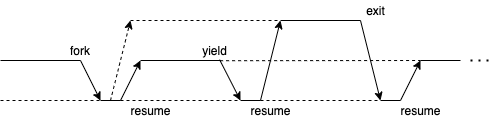
\includegraphics[width=0.8\textwidth]{imgs/scheduleBF.png}
    \caption{Breadth-First scheduling}\label{fig:scheduleBF}
  \end{subfigure}
  \begin{subfigure}
    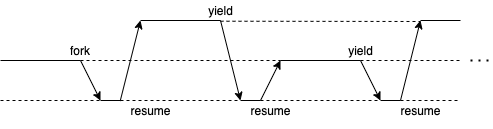
\includegraphics[width=0.8\textwidth]{imgs/scheduleDF.png}
    \caption{Depth-First scheduling}\label{fig:scheduleDF}
  \end{subfigure}
\end{figure}

\chapter{Formalisation of Frank}
\label{chap:formalisation}

%% We now discuss the formalisation of the Frank language. This has been discussed
%% in depth in previous work (\cite{convent2020doo}), so we do not go into great
%% detail about some parts of the language. Indeed, we skip over much of it for
%% brevity's sake. We do, however ht

The formalisation of the Frank language has been discussed at length in previous
work~(\cite{convent2020doo}). However, in order to illustrate changes made to
the language to get pre-emptive concurrency, we explain some of the key parts of
the language in this section.

\begin{figure}[h]  %\figrule
\[
\ba{@{}c@{}}
\ba{@{}c@{\quad\quad}c@{}}
\begin{syn}
  \slab{data types}            & D \\
  \slab{value type variables}  & X \\
  \slab{effect type variables} & E| \\
  \slab{value types}           & A, B   &::= & D~\overline{R} \\
                               &        &\gor& \thunk{C} \gor X \\
  \slab{computation types}     & C      &::= & \many{T \to}~G \\
  \slab{argument types}        & T      &::= & \effin{\adj}A \\
  \slab{return types}          & G      &::= & \effout{\sigs}A \\

  \slab{type binders}          & Z      &::= & X \gor [E]\\
  \slab{type arguments}        & R      &::= & A \gor [\Sigma]\\
  \slab{polytypes}             & P      &::= & \forall \overline{Z}.A \\
\end{syn}
&
\begin{syn}
  \slab{interfaces}           & I \\
  \slab{term variables}       & x, y, z, f \\
  \slab{instance variables}   & \pid, a, b, c \\
  \slab{seeds}                & \seed  &::= & \nowt \gor \ev \\
  \slab{abilities}            & \sigs  &::= & \seed\pipe\ext \\
  \slab{extensions}           & \ext   &::= & \id \gor \ext, \sig~\many{R} \\
  \slab{adaptors}             & \adapt &::= & \id \gor \adapt, \sig(S \to S') \\
  \slab{adjustments}          & \adj   &::= & \adapt\pipe\ext \\
  \slab{instance patterns}    & S      &::= & \pid \gor S \snoc a \\
  \slab{kind environments}    & \kenv,
                                \kenva &::= & \cdot \gor \kenv, Z \\
  \slab{type environments}    & \Gamma &::= & \cdot \gor \Gamma, x:A %\\
%                              &        &    & \hphantom{\cdot}
                                              \gor \Gamma, f:P\\
 \slab{instance environments} & \ienv  &::= & \pid:\sigs \gor \ienv, a:\sig~\many{R}\\
\end{syn} \\
\ea \\
\ea
\]
\\[0.25cm]

\caption{Types}
\label{fig:types}
%\figrule
\end{figure}

Value types are either datatypes instantiated with type arguments $D~\overline{R}$, thunked
computations $\thunk{C}$, or value type variables $X$. Computation types are
zero or more argument types $T$ resulting in a return type $G$. A computation of
type

\[
C = \effin{\adapt_1\pipe\ext_1}A_1 \to \dots \to
      \effin{\adapt_k\pipe\ext_k}A_k \to \effout{\sigs}B
\]

has arugment types $\effin{\adapt_i\pipe\ext_i}A_i$ and return type
$\effout{\sigs}B$; that is, a computation of type $C$ handles effects in
extensions $\ext_i$ in its $i$-hth argument. It then returns a value of type $B$
and potentially performs effects in $\sigs$.

\todo{Talk about adaptors at each index?}

An ability $\sigs$ \ldots. It may be closed $\nowt$ or open $\ev$.
%
An extension $\ext$ is a finite list of interfaces.

We deliberately leave out details on adaptors for the sake of brevity. We also
skip over the typing rules, as they are standard. These can be seen in the
appendix.

\begin{figure} %\figrule
\begin{syntax}
  %% \slab{monomorphic term variables} & x, y, z \\
  %% \slab{polymorphic term variables} & f \\
  \slab{constructors}               & k \\
  \slab{commands}                   & c \\
  \slab{uses}                 & m      &::= &
     x \gor f~\many{R} \gor m~\many{n} \gor \cu(n:A) \\
  \slab{constructions}        & n      &::= &
    \uc m \gor k~\many{n} \gor c~\many{R}~\many{n} \gor \thunk{e} \\
                              &        &\gor& \key{let}~f : P = n~\key{in}~n'
                                   \gor
                                   \key{letrec}~\many{f : P = e}~\key{in}~n \\
                              &        &\gor&  \effin{\adapt}~n \\
  \slab{computations}         & e      &::=& \many{\many{r} \mapsto n}
  \\
  \slab{computation patterns} & r      &::=& p
                                        \gor \effin{\handle{c~\many{p}\,}{z}}
                                        \gor \effin{x} \\
  \slab{value patterns}       & p      &::=& k~\many{p} \gor x        \\
\end{syntax}
\\[0.25cm]
%\textit{with} term variables $x$, $y$, $z$, polymorphic term variables $f$, constructors $k$, commands $c$\\[0.25cm]
\caption{Terms}
\label{fig:terms}
% \figrule
\end{figure}

\paragraph*{Terms} Frank uses bidirectional typing (\cite{pierce2000local}); as such, terms are
split into \emph{uses} whose types are inferred, and \emph{constructions}, which
are checked against a type. Uses are monomorphic variables $x$, polymorphic
variable instantiations $f~\many{R}$, applications $m~\many{n}$ and type
ascriptions $\cu(n:A)$. Constructions are made up of uses $\uc m$, data
constructor instances $k~\many{n}$, suspended computations $\thunk{e}$, let
bindings $\key{let}~f : P = n~\key{in}~n'$, recursive let $\key{letrec}~\many{f
  : P = e}~\key{in}~n$ and adaptors $\effin{\adapt}~n$. We can inject a use into
a construction with $\uc$ and vice versa ($\cu$); in real Frank code these are
not present.

Computations are produced by defining a sequence of pattern matching clauses.
Each pattern matching clause takes a sequence $\many{r}$ of computation
patterns. These can either be a request pattern
$\effin{\handle{c~\many{p}\,}{z}}$, a catch-all pattern $\effin{x}$, or a
standard value pattern $p$. Value patterns are made up of data constructor
patterns $k~\many{p}$ or variable patterns $x$.

\todo{Talk about typing for Frozen commands --- basically jus say that they
  retain the type when frozen.}

\paragraph*{Runtime Syntax}

The operational semantics uses the runtime syntax of
Figure~\ref{fig:runtime-syntax}. The uses and constructions are supplemented
with a special term $\freeze{\EC[c~\many{R}~\many{w}]}$, of \emph{frozen
  commands}. We discuss these further later.

We distinguish use and construction values, and then further separate
construction values into uses and non-uses. We also declare a new class of
\emph{normal forms}, to be used in pattern binding.

Finally we have evaluation contexts, which are sequences of evaluation frames.
The interesting case is $u~(\many{t}, [~],\many{n})$; it is this that gives us
left-to-right evaluation of multihandler arguments.

\begin{figure}[t]
%% \figrule
\begin{syntax}
\slab{uses}                    & m   &::= & \dots \mid \freeze{\EC[c~\many{R}~\many{w}]} \\
\slab{constructions}           & n   &::= & \dots \mid \freeze{\EC[c~\many{R}~\many{w}]} \\
\slab{use values}              & u   &::= & x \gor f~\many{R} \gor \cu (v : A) \\
\slab{non-use values}          & v   &::= & k~\many{w} \gor \thunk{e} \\
\slab{construction values}     & w   &::= & \uc u \gor v \\
\slab{normal forms}            & t   &::= & w \gor \freeze{\EC[c~\many{R}~\many{w}]} \\
\slab{evaluation frames}       & \EF &::= & [~]~\many{n}
                                      \gor  u~(\many{t},[~],\many{n})
                                      \gor  \cu([~]:A) \\
                               &     &\gor& \uc [~]
                                      \gor  k~(\many{w},[~],\many{n})
                                      \gor  c~\many{R}~(\many{w},[~],\many{n}) \\
                               &     &\gor& \key{let}~f: P = [~]~\key{in}~n
                                      \gor \effin{\adapt}~[~] \\
\slab{evaluation contexts}     & \EC &::= & [~] \gor \EF[\EC] \\
\end{syntax}
\caption{Runtime Syntax}
\label{fig:runtime-syntax}
%% \figrule
\end{figure}

\paragraph*{Operational Semantics} Finally, the operational semantics are given
in Figure~\ref{fig:operational-semantics}.

The essential rule here is \textsc{R-Handle}. This relies on a new relations
regarding \emph{pattern binding} (Figure~\ref{fig:pattern-binding}). We discuss
these rules in more detail later. $\bindsc{r}{T}{t}{\sigs}{\venv}$ states that
the computation pattern $r$ of type $T$ and ability $\sigs$ matches the normal
form $t$ yielding substitution $\venv$. The index $k$ is then the index of the
earliest ``line'' of pattern matches that all match. The conclusion of the rule
states that we then perform the substitutions $\many{\venv}$ that we get on the
return value $n_k$ to get our result. This is given type $B$.

\todo{Tighten up description.}

\textsc{R-Ascribe-Use} and \textsc{R-Ascribe-Cons} remove unneeded conversions
from use to construction. \textsc{R-Let} and \textsc{R-LetRec} are standard.
\textsc{R-Adapt} shows that an adaptor applied to a value is the identity.

We have several rules regarding the freezing of commands. When handling a
command, we need to capture its delimited continuation; that is, the largest
enclosing evaluation context that does \emph{not} handle it.
\textsc{R-Freeze-Comm} shows how commands, once used, become frozen;
\textsc{R-Freeze-Frame-Use} and \textsc{R-Freeze-Frame-Cons} show how the rest
of the context becomes frozen. These two rules rely on the predicate $\EC
\textsf{ handles } c$. This is true if the context does indeed handle the
command $c$; i.e. it is a context of the form $u~(\many{t}, [~], \many{u'})$
where $u$ is a handler that handles $c$ at the index corresponding to the hole.
Thus, the whole term is frozen up to the first handler, at which point is it
handled with \textsc{R-Handle}}.

The $\textsc{R-Lift}$ rules then express that we can perform any of these
reductions in any evaluation context.


\todo{Frozen commands - delimited continuations}

\begin{figure}[t]
%% \figrule
\flushleft
$\boxed{m \redtou m'} \quad \boxed{n \redtoc n'} \quad \boxed{m
    \stepstou m'} \quad \boxed{n \stepstoc n'}$
\begin{mathpar}
\inferrule[R-Handle]
  {% The type system should enforce this!
   %(\handles{\adj_j}{t_j})_j \\
   k = \min_i\,\{i \mid \exists \many{\venv}.(\bindsc{r_{i,j}}{\effin{\adj_j} A_j}{t_j}{\sigs}{\venv_j})_{j}\} \\
   (\bindsc{r_{k,j}}{\effin{\adj_j} A_j}{t_j}{\sigs}{\venv_j})_{j}}
   %% \forall i < k.\exists j.r_{i, j} \# t_j}
   %% l \text{~is minimal}}
  {\cu (\thunk{((r_{i,j})_j \to n_i)_i} : \thunk{\many{\effin{\adj} A \to}~\effout{\sigs}B})~\many{t} \redtou \cu ((\many{\venv}(n_k) : B)}

\inferrule[R-Ascribe-Use]
  { }
  {\cu(\uc u:A) \redtou u}

\inferrule[R-Ascribe-Cons]
  { }
  {\uc \cu (w : A) \redtoc w}

\inferrule[R-Let]
  { }
  {\key{let}~f:P = w~\key{in}~n \redtoc n[\cu (w : P)/f]}

\inferrule[R-LetRec]
  {\many{e = \many{\many{r} \to n}}}
  {%\vphantom{\many{\many{\many{\many{f}}}}}
   \key{letrec}~\many{f:P = e}~\key{in}~n' \redtoc
    n'[\many{\cu (\thunk{\many{\many{r} \to \key{letrec}~\many{f:P = e}~\key{in}~n}}: P)/f}]}

\inferrule[R-Adapt]
  { }
  {\effin{\adapt}~w \redtoc w}

\inferrule[R-Freeze-Comm]
  { }
  {c~\many{R}~\many{w} \redtoc \freeze{c~\many{R}~\many{w}}}\\

\inferrule[R-Freeze-Frame-Use]
  {\neg(\EF[\EC] \handles c)}
  {\EF[\freeze{\EC[c~\many{R}~\many{w}]}] \redtou \freeze{\EF[\EC[c~\many{R}~\many{w}]]}}

\inferrule[R-Freeze-Frame-Cons]
  {\neg(\EF[\EC] \handles c)}
  {\EF[\freeze{\EC[c~\many{R}~\many{w}]}] \redtoc \freeze{\EF[\EC[c~\many{R}~\many{w}]]}}

\\
\inferrule[R-Lift-UU]
  {m \redtou m'}
  {\EC[m] \stepstou \EC[m']}

\inferrule[R-Lift-UC]
  {m \redtou m'}
  {\EC[m] \stepstoc \EC[m']}

\inferrule[R-Lift-CU]
  {n \redtoc n'}
  {\EC[n] \stepstou \EC[n']}

\inferrule[R-Lift-CC]
  {n \redtoc n'}
  {\EC[n] \stepstoc \EC[n']}
\end{mathpar}

\caption{Operational Semantics}
\label{fig:operational-semantics}
%% \figrule
\end{figure}

\paragraph*{Pattern Binding}

We now discuss the pattern binding rules of Figure~\ref{fig:pattern-binding}.

\begin{figure}[t]
%% \figrule
\flushleft
%\textit{Comp. pattern $r$ for $\langle \Delta \rangle A$ matches $u$ under
%amb. $\venv$ and binds $\venv$.}
$\boxed{\bindsc{r}{T}{t}{\sigs}{\venv}}$
\begin{mathpar}

\inferrule[B-Value]
  {\adjact{\sigs}{\adj}{\sigs'} \\\\ \bindsv{p}{A}{w}{\venv}}
  {\bindsc{p}{\effin{\adj}A}{w}{\sigs}{\venv}}

  \inferrule[B-Request]
    {%I~\many{R} \in \ext \\ %\capturesI{\Delta}{I}{\iota}\\
    \adjact{\sigs}{\adj}{\sigs'} \\
    \EC \poised c \\\\
    \adj = \adapt\pipe\ext \\
    c : \forall \many{Z}. \many{B \to}~B' \in \ext \\
    (\bindsv{p_i}{B_i}{w_i}{\venv_i})_i}
    {\bindsc{\effin{c~\many{p} \to z}}{\effin{\adj}A}
    {\freeze{\EC[c~\many{R}~\many{w}]}}{\sigs}{\many{\venv}[\cu (\thunk{x \mapsto \EC[x]} : \thunk{B' \to \effout{\sigs'}A})/z]}}
\\
\inferrule[B-CatchAll-Value]
  {\adjact{\sigs}{\adj}{\sigs'}}
  {\bindsc{\effin{x}}{\effin{\adj}A}{w}{\sigs}{[\cu (\thunk{w}\mathord{:}\thunk{\effout{\sigs'}A})/x]}}
\\
\inferrule[B-CatchAll-Request]
  {
  \adjact{\sigs}{\adj}{\sigs'} \\
  \EC \poised c \\\\
  \adj = \adapt\pipe\ext \\
  c : \forall \many{Z}. \many{B \to}~B' \in \ext
  }
  {\bindsc{\effin{x}}{\effin{\adj}A}
  {\freeze{\EC[c~\many{R}~\many{w}]}}
  {\sigs}
  {[\cu (\thunk{\freeze{\EC[c~\many{R}~\many{w}]}}\mathord{:}\thunk{\effout{\sigs'}A})/x]}}

\end{mathpar}


%~~ \textit{Value pattern $p$ for type $A$ matches $w$ and binds $\venv$.}
%
$\boxed{\bindsv{p}{A}{w}{\venv}}$
\begin{mathpar}

\inferrule[B-Var]
  { }
  {\bindsv{x}{A}{w}{[\cu (w : A)/x]}}

\inferrule[B-Data]
  {k~\many{A} \in D~\many{R} \\
   (\bindsv{p_i}{A_i}{w_i}{\venv_i})_i}
 {\bindsv{k~\many{p}}{D~\many{R}}{k~\many{w}}{\many{\venv}}}
\end{mathpar}

\caption{Pattern Binding}
\label{fig:pattern-binding}
%% \figrule
\end{figure}



\chapter{Pre-emptive Concurrency}
\label{chap:preemptive-concurrency}

\section{Motivation}
\label{sec:interrupt-motivation}

One important part of our asynchronous effect handling system is the ability to
interrupt arbitrary computations. If two threads are running concurrently and
are communicating with one another, we have to stop running one to let messages
come in from the other. This is achievable with explicitly yielding, as in
Section~\ref{sec:concurrency}, however we would prefer for this behaviour to be
done automatically.

Consider the two programs below;

\begin{lstlisting}
controller : {[Stop, Go, Console] Unit}
controller! =
    stop!; print "stop "; sleep 200000; go!; controller!

runner : {[Console] Unit}
runner! = print ``1 ``; print ``2 ``; print ``3 '';
\end{lstlisting}

%% \noindent We ideally want a multihandler that can run these two programs in
%% parallel, such that the console output will be \code{1 stop 2 stop 3 stop}; that
%% is to say, the \code{stop} and \code{go} operations from \code{controller} can
%% control the execution of \code{runner}.

\noindent We want a multihandler that uses the \code{stop} and \code{go} commands from
\code{controller} to control the execution of \code{runner}. The console output
of this multihandler should be then \code{1 stop 2 stop 3 stop}.
%
%We need
%% pre-emptive interruptions for this, as otherwise there would be no way for the
%% \code{stop} and \code{go} messages to be registered.

\section{Interruption with Yields}
\label{sec:yield-interruption}

%% One way we can get this behaviour is using the \code{Yield} interface. This
%% offers a single operation, \code{yield : Unit}. With this, we can write a
%% multihandler \code{suspend};

We can simulate this behaviour by using the familiar \code{Yield} interface from
Section~\ref{subsec:simple-scheduling}.

\begin{lstlisting}
runner : {[Console, Yield] Unit}
runner! = print "1 "; yield!; print "2 "; yield!; print "3 "; yield!

suspend : {<Yield> Unit -> <Stop, Go> Unit
  -> Maybe {[Console, Yield] Unit} -> [Console] Unit}
suspend <yield -> r> <stop -> c> _ =
    suspend unit (c unit) (just {r unit})
suspend <_>          <go -> c>   (just res) =
    suspend res! (c unit) nothing
suspend unit         <_>         _ = unit
\end{lstlisting}

\noindent Running \code{suspend runner! controller! nothing} then prints out
\code{1 stop 2 stop 3} as desired.
%
This is due to the same synchronisation behaviour that we saw in
Section~\ref{subsec:simple-scheduling}; \code{runner} is evaluated until it
becomes a command or a value, and then \code{controller} is given the same
treatment. Once both are a command or a value, pattern matching is done.

This gives us the desired behaviour; the use of \code{yield} gives the
controller a chance to run, and also gives us access to the continuation of
\code{runner}. We can then use this to implement whatever scheduling strategy we
like.
%
We are, however, still operating co-operatively; the programmer has to manually
insert \code{yield} commands. If the programmer does not do so evenly enough
then either process could become starved. As such, we continue searching for a
better solution.

%% So far so good; this works as we hoped. However, observe that we had to change
%% the code of the \code{runner} to \code{yield} every time it prints.
%% %
%% %% We would rather not have this requirement; the threads should be suspendable
%% %% without knowing in advance they will be suspended, and thus without needing to
%% %% explicitly \code{yield}.
%% %
%% This is not in the spirit of pre-emptive concurrency; we are still operating
%% co-operatively. Threads should be unaware of the fact they are even being
%% pre-empted.
%% % The below line could maybe go...
%% Furthermore, see that the \code{yield} operation adds no more information; it is
%% just used as a placeholder operation; any operation would work.
%% %
%% As such, we keep searching for a better solution.

\section{Relaxing Catches}
\label{sec:relaxing-catches}

One approach is to relax the rules for pattern matching with the catchall
pattern $\effin{x}$. This would let us match generic commands that may not be
handled by the current handler. The key to implementing this lies in the pattern
binding rules of Figure~\ref{fig:pattern-binding}; specifically
\textsc{B-CatchAll-Request}.

%% The key to this lies in the catchall pattern, $\effin{x}$, and the pattern
%% binding rules of Figure~\ref{fig:pattern-binding}; specifically
%% \textsc{B-CatchAll-Request}. %We quickly go into detail on this rule now.
%
%% $\effin{x} : {\effin{\adj}A}$ states that $\effin{x}$ is a term with value type
%% $A$ and \emph{adjustment} $\adj = \adapt\pipe\ext$, made up of an adaptor
%% $\adapt$ and an extension $\ext$. This extension is made up of a list of
%% interface instantiations $\sig~\many{R}$.

The crux is that the command $c$ that is invoked in the frozen term
$\freeze{\EC[c~\many{R}~\many{w}]}$ must be a command offered by the extension
$\ext$; that is, it must be handled by the current use of \textsc{R-Handle}.
Refer back to the example of Section~\ref{sec:yield-interruption}. This rules
means that the catch-all pattern \code{<_>} in the final pattern matching case
of \code{suspend} can match against \code{stop} or \code{go}, as they are
present in the extension of the second argument, but not \code{print} commands;
although the \code{Console} interface is present in the ability of
\code{controller}, it is not in the extension in \code{suspend}.



%% Recall that the catchall pattern $\effin{x}$ matches either a value or a command
%% that is present in the term's ability. For instance, the pattern \code{<k>} in
%% the code above matches either \code{unit} or \code{<yield -> k>}. The variable
%% \code{k} is then bound to whatever this match is, leaving the (potentially)
%% invoked command unhandled. This is expressed in the \textsc{B-CatchAll-Request}
%% rule in Figure~\ref{fig:pattern-binding} (restated in
%% Figure~\ref{fig:loose-catchall-request}).

%% \todo{'Present in the term's ability' is incorrect, fix }


%% Important to note is that only effects that are handled in that position are
%% able to be caught. \code{runner} also makes use of the \code{print} effect, but
%% these are not able to be caught by the catchall command. Formally, this is due
%% to the fourth requirement of \textsc{B-CatchAll-Request}; that the command $c$
%% that is invoked is a member of $\ext$.

\begin{figure}[h]
%% \figrule
%% \flushleft
%% \centering
%\textit{Comp. pattern $r$ for $\langle \Delta \rangle A$ matches $u$ under
%amb. $\venv$ and binds $\venv$.}
\begin{mathpar}
%% \\
\inferrule[B-CatchAll-Request-Loose]
  {
  \adjact{\sigs}{\adj}{\sigs'} \\
  %% \EC \poised c \\\\
  %% \adj = \adapt\pipe\ext \\
  %% c : \forall \many{Z}. \many{B \to}~B' \in \ext
  }
  {\bindsc{\effin{x}}{\effin{\adj}A}
  {\freeze{\EC[c~\many{R}~\many{w}]}}
  {\sigs}
  {[\cu (\thunk{\freeze{\EC[c~\many{R}~\many{w}]}}\mathord{:}\thunk{\effout{\sigs'}A})/x]}}
\end{mathpar}
\caption{Updated \textsc{B-CatchAll-Request}}
\label{fig:loose-catchall-request}
%% \figrule
\end{figure}

In the interests of pre-emption, we propose to remove this constraint from
\textsc{B-CatchAll-Request}, replacing the rule with
\textsc{B-CatchAll-Request-Loose} as seen in
Figure~\ref{fig:loose-catchall-request}. This lets us update the previous
\code{suspend} code to the following, which yields the same results as last
time;

\begin{lstlisting}
runner : {[Console] Unit}
runner! = print "1 "; print "2 "; print "3 "

suspend : {Unit -> <Stop, Go> Unit -> Maybe {[Console] Unit} -> [Console] Unit}
suspend <r> <stop -> c> _ =
    suspend unit (c unit) (just r)
suspend <_>          <go -> c>   (just res) =
    suspend res! (c unit) nothing
suspend unit         <_>         _ = unit
\end{lstlisting}

\noindent Now when we run \code{suspend runner! controller! nothing}, the
\code{suspend} handler can match the catchall pattern \code{<r>} against the
\code{print} commands in \code{runner}.

The no-snooping policy with respect to effect handlers (\cite{convent2020doo})
states that a handler should not be able to intercept effects that it does not
handle. This change breaks this policy, as we can now tell when an command is
used. Whilst we can not handle it as per usual, we get the option to throw away
the continuation. A system that does not allow for snooping is much preferred.

\section{Freezing Arbitrary Terms}
\label{sec:freezing-terms}

The approach of Section~\ref{sec:relaxing-catches} can only interrupt command
invocations. If \code{runner} were instead a sequence of pure
computations\footnote{I.e. \code{runner! = 1 + 1; 1 + 1; 1 + 1}; $\ldots$} we would
be unable to interrupt it; it does not invoke commands.

As such, we need to further change the pattern binding rules of Figure
\ref{fig:pattern-binding}. This is to let us interrupt arbitrary computation
terms. In Figure~\ref{fig:runtime-syntax-freeze}, we see an updated version of
the runtime syntax; this allows for the suspension of arbitrary \emph{uses}.

\begin{figure}[t]
%% \figrule
\begin{syntax}
\slab{uses}                    & m   &::= & {\dots} \gor
\freeze{\EC[c~\many{R}~\many{w}]} \gor \highlight{\freeze{m}} \\
\slab{constructions}           & n   &::= & \dots \gor
\freeze{\EC[c~\many{R}~\many{w}]} \gor \highlight{\freeze{m}} \\
\slab{use values}              & u   &::= & x \gor f~\many{R} \gor \cu (v : A) \\
\slab{non-use values}          & v   &::= & k~\many{w} \gor \thunk{e} \\
\slab{construction values}     & w   &::= & \uc u \gor v \\
\slab{normal forms}            & t   &::= & w \gor \freeze{\EC[c~\many{R}~\many{w}]} \gor \highlight{\freeze{m}}\\
\slab{evaluation frames}       & \EF &::= & [~]~\many{n}
                                      \gor  u~(\many{t},[~],\many{n})
                                      \gor  \cu([~]:A) \\
                               &     &\gor& \uc [~]
                                      \gor  k~(\many{w},[~],\many{n})
                                      \gor  c~\many{R}~(\many{w},[~],\many{n}) \\
                               &     &\gor& \key{let}~f: P = [~]~\key{in}~n
                                      \gor \effin{\adapt}~[~] \\
\slab{evaluation contexts}     & \EC &::= & [~] \gor \EF[\EC] \\
\end{syntax}
\caption{Runtime Syntax, Updated with Freezing of Uses}
\label{fig:runtime-syntax-freeze}
%% \figrule
\end{figure}


\begin{figure}[h]
%% \figrule
\flushleft
$\boxed{m \redtou m'} \quad \boxed{n \redtoc n'}$
\begin{mathpar}

\inferrule[R-Freeze-Use]
  {  }
  { m \redtou \freeze{m} }

\inferrule[R-Freeze-Frame-Use]
  { \EF \textsf{ not handler }}
  { \EF[\EC[\freeze{m}]] \redtou \freeze{\EF[\EC[m]]} }

\inferrule[R-Freeze-Frame-Cons]
  { \EF \textsf{ not handler }}
  { \EF[\EC[\freeze{m}]] \redtoc \freeze{\EF[\EC[m]]} }

\end{mathpar}

\caption{Updated Freezing}
\label{fig:Freezing}
%% \figrule
\end{figure}

Note that frozen terms here behave in a similar way to frozen commands, by
freezing the rest of the term around it as well. This continues up until a
handler is reached, at which point the term is unfrozen and resumed. This
process of freezing up to a handler is enforced by the predicate $\EF \textsf{
  not handler }$, which is true only when $\EF$ is of the form $u~(\many{t},
[~], \many{n})$.

With this in mind, we now give the updated rule for the catchall pattern
matching on frozen terms. This can be seen in Figure \ref{fig:catchall-freeze}.
It expresses that an arbitrary frozen term can be matched against the
computation pattern $\effin{x}$. The suspended, unfrozen computation $\thunk{m}$
is then bound to $x$, in a similar way to other \textsc{B-CatchAll} rules.
Observe that this maintains no-snooping; we don't know that the frozen
computation performed an effect.

\begin{figure}[t]
%% \figrule
\flushleft
%\textit{Comp. pattern $r$ for $\langle \Delta \rangle A$ matches $u$ under
%amb. $\venv$ and binds $\venv$.}
\begin{mathpar}
\inferrule[B-CatchAll-Freeze]
  {\adjact{\sigs}{\adj}{\sigs'}}
  {\bindsc{\effin{x}}{\effin{\adj}A}{\freeze{m}}{\sigs}{[\cu (\thunk{m}\mathord{:}\thunk{\effout{\sigs'}A})/x]}}
\end{mathpar}

\caption{Catching Interrupts rule. }
\label{fig:catchall-freeze}
%% \figrule
\end{figure}

%% \begin{lstlisting}
%% suspend : {Unit -> <Stop, Go> Unit -> Maybe {[Console] Unit} -> [Console] Unit}
%% suspend <r> <stop -> c> _ =
%%     suspend unit (c unit) (just r)
%% suspend <_>          <go -> c>   (just res) =
%%     suspend res! (c unit) nothing
%% suspend unit         <_>         _ = unit
%% \end{lstlisting}

We can simply reuse the \code{suspend} handler from
Section~\ref{sec:relaxing-catches}. Everything works largely the same; we run the
leftmost argument until it freezes or invokes a command, at which point we run
the next argument. The frozen term can then be bound to the catch-all pattern, if
this is the pattern that matches.


\section{Yielding}
\label{sec:inserting-yields}

Observe that the freezing approach of Section~\ref{sec:freezing-terms} ends up
reimplementing a lot of the behaviour of the freezing of ordinary commands,
without adding much new behaviour. It turns out that we can get the exact same
behaviour by just inserting a command invocation into the term instead, and
handling this as normal.
%
%% This
%% will also freeze the computation up until the nearest handler of the inserted
%% command.

%% We use the familair \Yield~effect from Section~\ref{sec:concurrency} for this
%% task.

%% Observe that the approach of Section~\ref{sec:relaxing-catches} can only
%% interrupt command invocations. If \code{runner} were instead a sequence of pure
%% computations\footnote{I.e. \code{runner! = 1 + 1; 1 + 1; 1 + 1; ...}}, we would
%% be unable to interrupt it; it does not invoke commands. In this section we show
%% how we can easily interrupt \emph{arbitrary terms}, without defining any special
%% new syntax or constructions. Furthermore, we do this in a
%% way that lets the programmer choose how to resume the term, without being set in
%% stone.

Recall the simple \Yield~effect from Section~\ref{sec:concurrency}; it
supports one operation, $\yield : \textsf{Unit}$.
%
Whilst it sounds boring from the type, remember that the invocation of an effect
offers up the continuation of the program as a first-class value, so that they
might concurrently run the function with other functions or control execution by
some other means.

Our solution is simple; whenever we are in an evaluation context where the
ability contains the \Yield effect, we insert an invocation of \yield before the
term in question. This is expressed formally in Figure~\ref{fig:insert-yield}.
We refer to this system as \nondetfrank.

\todo{Add rules for eval ctxs converting use to const, use to use, etc}

\begin{figure}[h]
%% \figrule
\flushleft
$\boxed{n \redtou n'} $
\begin{mathpar}
%
%
\inferrule[R-Yield-EF]
          { \EC~\textsf{allows}~\yield }
          { \EC[n] \redtou \EC[\textsf{yield!}; n] }
\end{mathpar}
%
%
\caption{Inserting Yields}
\label{fig:insert-yield}
%% \figrule
\end{figure}

%% Note that \textsc{R-Yield-EF} relies on the predicate
%% $\EF[\EC]~\allows~c$. This states that the \yield
%% interface is in the ability of the term in the evaluation context.

Note that \textsc{R-Yield-EF} relies on the predicate $\EC~\allows~c$. For any
frame apart from argument frames, $\EF[\EC]~\allows~c = \textsf{false}$. In this
case, it is defined as follows;

\begin{align*}
  \cu (v : \thunk{\many{\effin{\adj} A
      \to}~\effout{\sigs}B})~(\many{t},[~],\many{n})~\allows~c =
  &~\ext_{|\many{t}|}~\allows~c ~ \\
  & \text{where}~\adj_{|\many{t}|} = \adapt_{|\many{t}|}\pipe\ext_{|\many{t}|}% \adjact{\sigs}{\adj_{|\many{t}|}}{\sigs'}
\end{align*}


%% \noindent For an ability $\sigs = \seed\pipe\ext$, the predicate $\sigs~ \allows~c$ is true if
%% $c \in I$ for some $I \in \ext$.

\noindent For an extension $\ext$, the predicate $\ext~\allows~c$ is true if $c
\in I$ for some $I \in \ext$.

Informally, $\EC~\allows~c$ is true when $\EC$ is a handler, and the extension at
the hole contains an interface which offers \yield~as a command. For instance,
if a handler had type \code{\{<Yield>X -> Y -> [Yield]X\}}, the first argument
would be allowed to yield but the second would not.

We also make use of an auxiliary combinator $\_ ; \_$. This is the traditional
sequential composition operator $\textsf{snd}~x~y~\mapsto~y$, where both
arguments are evaluated and the result of the second one is returned. We see
that it would be a type error if we were to insert a \code{yield} command in a
context where \yield~was not a part of the ability. In the context of
\textsc{R-Yield-EF} this means we will perform the \yield~operation and then the
use $m$, but discard the result from \yield.

Observe that this gives us fine-grained control over which parts of our program
become asynchronous. One might want a short-running function to not be
pre-emptible and just run without pause; conversely, one might want a
long-running function to be interruptible. The programmer gets to choose this by
labelling the functions with \yield in the ability. This is one improvement over
the system of Section~\ref{sec:freezing-terms}, another being that we define
fewer new rules and constructs.

%% \todo{Talk about how this differs to the Freezing system}.

\paragraph*{Nondeterminism}

Observe that this system, and the system from Section~\ref{sec:freezing-terms},
are both nondeterministic. This is because at any point we have the opportunity
to either invoke yield (respectively freeze the term), or continue as before.

Consider running \code{hdl (print "A") (print "B")}, for some binary
multihandler \code{hdl}. We could evaluate
\code{print "A"} first and then \code{print "B"}, or freeze \code{print "A"} and
evaluate \code{print "B"} first. Both of these would obviously result in
different things printed to the console.

\section{Counting}

The semantics given by Section~\ref{sec:inserting-yields} is fine, but is
non-deterministic; at any point, we can choose to either insert a \yield
invocation or carry on as normal. Furthermore, we do not particularly need to
yield very frequently; we might rather yield every 1000 reduction steps or so.

As such, we supplement the operational semantics with a counter $\counter$. This
counter has two states; it could either be counting up, which is the form
$\justc{n}$ for some $n$, or it is a signal to yield as soon as possible, which
is the form $\yieldc$.

To increment this counter, we use a slightly modified version of addition,
denoted $\plusc$. This is simply defined as

\begin{equations}
  x \plusc y =
          \left\{ \ba{@{}l@{\quad}l@{}}
              \justc{x + y} & \text{if } x + y \leq \threshc \\
              \yieldc & \text{otherwise}
          \right.
\end{equations}

\noindent where $\threshc$ is the threshold at which we force a yield.

The transitions in our operational semantics now become of the form $m; \counter
\redtou m'; \counter '$. In Figure~\ref{fig:counting-rules} we give an updated
rule for \textsc{R-Handle} --- overwriting the previous rule --- and two new
rules for inserting yields. We refer to this system as \countingfrank.

\begin{figure}
%% \figrule
\flushleft
$\boxed{m \redtou m'} \quad \boxed{n \redtoc n'} \quad \boxed{m
    \stepstou m'} \quad \boxed{n \stepstoc n'}$
\begin{mathpar}
\inferrule[R-Handle-Count]
  {% The type system should enforce this!
   %(\handles{\adj_j}{t_j})_j \\
   k = \min_i\,\{i \mid \exists \many{\venv}.(\bindsc{r_{i,j}}{\effin{\adj_j} A_j}{t_j}{\sigs}{\venv_j})_{j}\} \\
   (\bindsc{r_{k,j}}{\effin{\adj_j} A_j}{t_j}{\sigs}{\venv_j})_{j}}
   %% \forall i < k.\exists j.r_{i, j} \# t_j}
   %% l \text{~is minimal}}
  {\cu (\thunk{((r_{i,j})_j \to n_i)_i} : \thunk{\many{\effin{\adj} A
        \to}~\effout{\sigs}B})~\many{t}; \justc{n}~
    \redtou~
    \cu ((\many{\venv}(n_k) : B)); n \plusc 1}

\\
\inferrule[R-Yield-Can]
          { \EC~\textsf{allows}~\yield }
          { \EC[m]; \yieldc~\redtou~\EC[\textsf{yield!}; m]; \justc{0} }
\\
\inferrule[R-Yield-Can't]
          { \neg (\EC~\textsf{allows}~\yield) \\
            m; \justc{n} \redtou m'; c' }
          { \EC[m]; \yieldc~\redtou~\EC[m]; \yieldc }
\\

\end{mathpar}

\caption{Yielding with Counting}
\label{fig:counting-rules}
%% \figrule
\end{figure}

\textsc{R-Handle-Count} replaces the previous rule \textsc{R-Handle}. If the
counter is in the state $\justc{n}$, we perform the handling as usual,
incrementing the counter by 1. Here we use $\plusc$, which will set the counter
to be $\yieldc$ if the addition brings it over the threshold value.

\textsc{R-Yield-Can} and \textsc{R-Yield-Can't} dictate what to do if we have to
yield as soon as possible. If the evaluation context allows \yield~
commands to be inserted we do so and reset the counter. If not, but the term
could otherwise reduce if the counter had a different value, then we make that
transition, still maintaining the $\yieldc$ signal.

\citeauthor{dolan2017concurrent} take a similar approach to this when
investigating asynchrony in Multicore OCaml (\cite{dolan2017concurrent}). They
rely on the operating system to provide a timer interrupt, which is handled as a
first-class effect. Our system is more self-contained; the timing is implemented
within the language itself and doesn't rely on the operating system providing
interrupts. Furthermore, we get fine-grained control over when the timer can
fire, as we can choose to put \yield~in the ability of interruptible
terms.

\paragraph*{Determinism}
Observe that the semantics of Frank equipped with the rules in
Figure~\ref{sec:counting-rules} are now deterministic; for any term and counter
pair, there is only one possible reduction we can make. This is a clear
improvement on the nondeterministic semantics of Section~\ref{sec:inserting-yields},
whilst still maintaining a similar behaviour; we are simply \emph{restricting}
the parts of the program where we can yield.

We can characterise this by saying that \countingfrank~\emph{implements}~
\nondetfrank; that is to say the counting system gives a deterministic way to
perform the nondeterministic system.

\begin{theorem}[Counting Implements Nondeterminism]
%% \begin{restatable}[Counting Implements Nondeterminsim]{theorem}{countimplynondet}\label{thm:count-impl-nondet}
\begin{itemize}
\item For any use $m$ and counter $\counter$, if $m, \counter~\redtou~
  m',\counter'$ in \countingfrank~ then $m~\redtou~m'$ in \nondetfrank.
\item For any construction $n$ and counter $\counter$, if $n, \counter~\redtou~
  n',\counter'$ in \countingfrank~ then $n~\redtou~n'$ in \nondetfrank.
\end{itemize}
%% \end{restatable}
\end{theorem}

One might consider a different approach, rather than a global counter, which
would also implement the nondeterministic semantics.

\section{Handling}
\label{sec:handling}

Observe that we can now use the same \code{suspend} handler from
Section~\ref{sec:interruption-with-yields}, without having to manually insert
\yield~commands in \code{runner}. Assuming the threshold $\threshc$ is set to 1, the
following code will give the desired output.

\begin{lstlisting}
runner : {[Console] Unit}
runner! = print "1 "; print "2 "; print "3 "

suspend : {<Yield> Unit -> <Stop, Go> Unit
  -> Maybe {[Console, Yield] Unit} -> [Console] Unit}
suspend <yield -> r> <stop -> c> _ =
    suspend unit (c unit) (just {r unit})
suspend <_>          <go -> c>   (just res) =
    suspend res! (c unit) nothing
suspend <yield -> r> <c>           = suspend (r unit) c!
suspend unit         <_>         _ = unit
\end{lstlisting}

\begin{lstlisting}
  suspend <yield -> k> a = blah
\end{lstlisting}

The first argument is evaluated until the counter is greater than the threshold,
at which point a yield command is performed; the rest of the computation is then
frozen and the second argument is evaluated. Observe that the \Yield interface
is not present in the adjustment of the second argument, so it is left to run
as normal.

We might also want to make the controller --- being the second argument ---
preemptible; it might do some other long-running computation in between
performing \code{stop} and \code{go} operations. We have to add \Yield to the
adjustment at the second argument, but also more pattern matching cases.

\begin{lstlisting}[
    linebackgroundcolor={%
        \btLstHL{7-9}}]
suspend : {<Yield> Unit -> <Stop, Go, <@\texthighlight{Yield}@>> Unit
  -> Maybe {[Console, Yield] Unit} -> [Console] Unit}
suspend <yield -> r> <stop -> c> _ =
    suspend unit (c unit) (just {r unit})
suspend <_>          <go -> c>   (just res) =
    suspend res! (c unit) nothing
<@\texthighlight{
suspend <yield -> r> <yield -> c>  = suspend (r unit) (c unit)
}@>
<@\texthighlight{
suspend <yield -> r> <c>           = suspend (r unit) c!
}@>
<@\texthighlight{
suspend <r>          <yield -> c>  = suspend r! (c unit)
}@>
suspend unit         <_>         _ = unit
\end{lstlisting}

These let \yield~commands synchronise with each other, achieving fair scheduling,
as discussed in Section~\ref{sec:concurrency}. It is a bit annoying to write
these by hand, as they take up a lot of space and are orthogonal to the rest of
the logic of the handler.

It is fortunate then that this process of resuming as many yields as possible
can be automated completely. Given a multihandler with $m$ arguments, $n$ of
which have \Yield~in their adjustment, we first try and resume all $n$
\yield~commands. After this we try and resume all of the different permutations
of $n-1$ \yield~commands, and so on until we are trying to resume 0
\yield~commands. The resuming clauses for the 3-ary case can be seen below.

\begin{lstlisting}
sch3 : {<Yield> Unit -> <Yield> Unit -> <Yield> Unit -> Unit}
sch3 <yield -> h> <yield -> j> <yield -> k> =
    sch3 (h unit) (j unit) (k unit)

sch3 <yield -> h> <yield -> j> <k> = sch3 (h unit) (j unit) k!
sch3 <yield -> h> <j> <yield -> k> = sch3 (h unit) j! (k unit)
sch3 <h> <yield -> j> <yield -> k> = sch3 h! (j unit) (k unit)

sch3 <yield -> h> <j> <k> = sch3 (h unit) j! k!
sch3 <h> <yield -> j> <k> = sch3 h! (j unit) k!
sch3 <h> <j> <yield -> k> = sch3 h! j! (k unit)
\end{lstlisting}

These commands can then be inserted generically at runtime. If no other
hand-written patterns match, we insert these patterns and try all of these. It
is important to try these after the rest of the patterns, as the use may want to
handle \yield~commands some other way; we do not want to interfere with this.
This means we can program in a direct manner manner, easily toggling which
arguments should be interruptible by adding \Yield~to the corresponding interface.

Automatically inserting \yield-handling clauses when combined with automatically
\emph{inserting} \yield~commands then gives us pre-emptive concurrency at no
overhead to the programmer.


\section{Soundness}

We now state the soundness property for our extended system, as well as the
subject reduction theorem needed for this proof. Our system is nothing more than
the system of~\citeauthor{convent2020doo} with extra rules; as such we omit most of
the details.


\begin{theorem}[Subject Reduction]\label{thm:sub-red}
\vskip
\begin{itemize}\\
\item If $\inferskgs{m}{A}$ and $m; \counter \redtou m'; \counter'$ then $\inferskgs{m'}{A}$.
\item If $\checkskgs{A}{n}$ and $n; \counter \redtoc n'; \counter'$ then $\checkskgs{A}{n'}$.
\end{itemize}
  \end{theorem}

\begin{proof}
The proof follows by induction on the transitions $\redtou, \redtoc$. We first
consider the two possible states for $\counter$. If it is in the form
$\justc{n}$, then the reduction rules are simply the same as
in~\cite{convent2020doo}, as we do not change the counter. The only exception to
this is the updated \textsc{R-Handle} rule, which is the same as before except
for modifications to the counter; regardless of the counter, the resulting term
$m'$ still remains the same type.

Thus the only new cases are \textsc{R-Yield-Can} and \textsc{R-Yield-Can't}.

\begin{itemize}
\item[\Cse] \textsc{R-Yield-Can}
  By the assumption we have that $\EC~\allows~\yield$. This only holds
  if the context is of the form
  \[\EC[~] = \cu (v : \thunk{\many{\effin{\adj} A
      \to}~\effout{\sigs}B})~(\many{t},[~],\many{n'})\]

  Assume that
  \[\inferskgs{\cu (v : \thunk{\many{\effin{\adj} A
      \to}~\effout{\sigs}B})~(\many{t},\EC'[n],\many{n'})}{B}\]

  From $\EC~\allows~\yield$ we know that $\yield \in \ext_{|\many{t}|}$ where
  $\adj_{|\many{t}|} = \adapt_{|\many{t}|}\pipe\ext_{|\many{t}|}$.
  %
  Then by inversion on \textsc{T-App} we have
  $\checksk{\Gamma}{\sigs'_{|\many{t}|}}{A_{|\many{t}|}}{\EC'[n]}$ and
  $\adjact{\sigs}{\adj_{|\many{t}|}}{\sigs_{|\many{t}|}}$.
  %
  It follows than that
  $\checksk{\Gamma}{\sigs'_{|\many{t}|}}{A_{|\many{t}|}}{\EC'[\yield; n]}$, as
  we know that \yield~commands are permitted under ability $\sigs'_{|\many{t}|}$.
  %

  %% This follows from the assumption $\EC~\allows~\yield$, which
  %% entails that $\yield~\in~\sigs'_{|\many{t}|}$. Thus
  %% $\inferskgs{\EC[\yield; n]}{B}$.

\item[\Cse] \textsc{R-Yield-Can't}
  This case is more straightforward. By the assumption we have that the
  evaluation frame $\EF$ does not permit yielding, but the term inside the frame
  could otherwise reduce.

  Assume $\checkskgs{A}{\EF[n]}$, and therefore $\checkskgs{A'}{n}$. By the
  assumption and subject reduction, $\checkskgs{A'}{n'}$. Then clearly
  $\checkskgs{A}{\EF[n']}$.

\end{itemize}
\end{proof}




\begin{theorem}[Type Soundness]\label{thm:soundness}
\begin{itemize}
\\
\item If $\infers{\cdot}{\cdot}{\sigs}{m}{A}$ then either $m$ is a normal form
  such that $m$ respects $\sigs$ or there exists a unique
  $\infers{\cdot}{\cdot}{\sigs}{m'}{A}$ such that $m \stepstou m'$.
\item If $\checks{\cdot}{\cdot}{\sigs}{A}{n}$ then either $n$ is a normal form
  such that $n$ respects $\sigs$ or there exists a unique
  $\checks{\cdot}{\cdot}{\sigs}{A}{n'}$ such that $n \stepstoc n'$.
\end{itemize}
%% In particular, if $\sigs = \nowt$ then either the term is a value $w$ or the
%% term can reduce by one step.
\end{theorem}

\begin{proof}
The proof proceeds by simultaneous induction on
$\infers{\cdot}{\cdot}{\sigs}{m}{A}$ and $\checks{\cdot}{\cdot}{\sigs}{A}{n}$.
\end{proof}

\todo{Talk about Soundness for \nondetfrank~as well as \countingfrank.}





%%%%%%%%%%%%%%%%%%%%%%%%%%%%%%%%%%%%%%%%%%%%%%%%%%%%%%%%%%%%%%%%%%%%%%%%%%%%%%%%%%%
%%%%%%%%%%%%%%%%%%%%%%%%%%%%%%%%%%%%%%%%%%%%%%%%%%%%%%%%%%%%%%%%%%%%%%%%%%%%%%%%%%%
%%%%%%%%%%%%%%%%%%%%%%%%%%%%%%%%%%%%%%%%%%%%%%%%%%%%%%%%%%%%%%%%%%%%%%%%%%%%%%%%%%%
%%%%%%%%%%%%%%%%%%%%%%%%%%%%%%%%%%%%%%%%%%%%%%%%%%%%%%%%%%%%%%%%%%%%%%%%%%%%%%%%%%%
%%%%%%%%%%%%%%%%%%%%%%%%%%%%%%%%%%%%%%%%%%%%%%%%%%%%%%%%%%%%%%%%%%%%%%%%%%%%%%%%%%%
%%%%%%%%%%%%%%%%%%%%%%%%%%%%%%%%%%%%%%%%%%%%%%%%%%%%%%%%%%%%%%%%%%%%%%%%%%%%%%%%%%%
%%%%%%%%%%%%%%%%%%%%%%%%%%%%%%%%%%%%%%%%%%%%%%%%%%%%%%%%%%%%%%%%%%%%%%%%%%%%%%%%%%%
%%%%%%%%%%%%%%%%%%%%%%%%%%%%%%%%%%%%%%%%%%%%%%%%%%%%%%%%%%%%%%%%%%%%%%%%%%%%%%%%%%%
%%%%%%%%%%%%%%%%%%%%%%%%%%%%%%%%%%%%%%%%%%%%%%%%%%%%%%%%%%%%%%%%%%%%%%%%%%%%%%%%%%%

\chapter{Implementation}
\label{chap:implementation}

We now introduce the Frank library used for asynchronous effects.
%
Our design closely follows the design of \aeff~(\cite{ahman2020asynchronous}), a
language designed around writing multithreaded programs that communicate by
sending \emph{interrupts}. A thread dictates how it will respond to an interrupt
by installing an \emph{interrupt handler}, also known as a \emph{promise}.
%
%% These are analogous to traditional effects and handlers; an interrupt when
%% invoked is like the invocation of a command, and an interrupt handler is like an
%% effect handler.
Interrupts and interrupt handlers can be seen as a less expressive version of
effects and effect handlers; an interrupt handler describes how to behave on
receipt of an interrupt in the same way to an effect handler, but it does not
get access to the continuation of the calling code.

Interrupts and interrupt handlers have one particularly compelling feature; when
we invoke an interrupt (in the case of synchronous effects, this is just
invoking a command), we can carry on computing the rest of the code whilst we
wait for a response. This is a stark difference to normal effects, where the
rest of the computation is blocked whilst we wait for an answer. The programmer
can then choose to await the response from interrupt, which blocks
computation until the interrupt handler has been fulfilled.

Unlike \aeff, our system does not track the uses of asychronous effects. It
does, however, track the traditional effects that are permitted in promises.

%% Our system is untyped in that there is no tracking of which asynchronous effects
%% are issued however it is typed in that the traditional Frank effects promises
%% can perform are tracked.

%% \aeff~has an effect tracking system for asynchronous effects; our system does
%% not. Ours does however track the effects that can be performed by interrupt
%% handlers.

\section{In Frank}

\aeff's interrupt handlers are manifested in Frank through the \code{Promise}
interface.

%% \begin{lstlisting}
%% interface Promise <@\greytext{[E]}@> =
%%       promise R : Prom R <@\greytext{[E | Promise[E|], RefState, Yield]}@>
%%                -> Pid R  <@\greytext{[E | Promise[E|], RefState, Yield]}@>
%%     | signal : Sig -> Unit
%%     | await R : Pid R <@\greytext{[E | Promise[E|], RefState, Yield]}@> -> R

%% data Prom R <@\greytext{[E]}@> = prom {Sig -> Maybe {<@\greytext{[E|]}@>R}}

%% data Pid X = pid (Ref (PromiseStatus X))

%% data PromiseStatus X = empty | done X | resume {X -> Unit}
%% \end{lstlisting}

\begin{lstlisting}
interface Promise =
      promise R : Prom R <@\greytext{[Promise, RefState, Yield]}@>
               -> Pid R  <@\greytext{[Promise, RefState, Yield]}@>
    | signal : Sig -> Unit
    | await R : Pid R <@\greytext{[Promise, RefState, Yield]}@> -> R

data Prom R <@\greytext{[E]}@> = prom {Sig -> Maybe {<@\greytext{[E|]}@>R}}

data Pid X = pid (Ref (PromiseStatus X))

data PromiseStatus X = waiting | done X | resume {X -> Unit}
\end{lstlisting}

\noindent The \code{promise R} command is a polymorphic command, which takes a
function of type \code{Sig -> Maybe \{[E|] R\}}. This function is an interrupt
handler; it dictates what to do on receipt of an interrupt, which is a thing of
type \code{Sig}. The return type of the interrupt handler is \code{Maybe \{[E|]
  R\}}; this is because the programmer has the chance to return \code{nothing},
which will mean the promise goes unfulfilled and waits for another message. The
programmer would want to do this on receipt of other types of message, or if a
certain condition regarding the interrupt is not fulfilled\footnote{Interrupt
  handlers which put conditions on the incoming interrupts are called
  \emph{guarded} interrupt handlers --- we come back to these later.}. An
interrupt handler corresponding to an asynchronous division could be;

\begin{lstlisting}
  div : {Sig -> Maybe {[Promise] Unit}}
  div (ask n d) = if (n > 0)
                     {just {signal (response (n / d))}}
                     {nohing}
  div _ = nothing
\end{lstlisting}

\noindent We call the thunk \code{signal (response (n / d))} the \emph{body} of
the interrupt handler. We say that an interrupt handler \emph{fires} if an
interrupt is received that results in a non-\code{nothing} value. Observe that
whilst we can perform some computation when deciding whether or not to fire
based on an interrupt, the type of \code{Prom R} restricts us so that we cannot
perform any effects whilst deciding; we may only perform effects in the body of
the promise.

The \code{promise R} operation returns a \code{Pid R}. This contains information
about the status of the promise; it is either empty, to signify the promise is
unfulfilled, or it holds the result of the promise, or it holds a resumption
that is automatically invoked when the promise is finished. Importantly, a
function installing a promise should not have access to the body of this; it
would ideally be some abstract type. The calling function should only interact
with the \code{Pid} through the \code{await} command.

\code{signal} is a more simple operation. The \code{Sig} data type is the type
of signals that the thread can invoke. These can hold extra data, also called a
\emph{payload}. For instance, if we had a program running remote function calls,
we might have \code{Sig = call ArgsType | result ResultType}. The handler
for \code{Promise} will then send the signals to each other thread, possibly
executing the interrupt handler if needs be.

\code{await} takes a \code{Pid R} and returns a value of type \code{R}. This
\code{R} is the returned value of the promise. \code{await} will block until the
promise it awaits has been fulfilled; we come on to how it does so later.

\paragraph*{Effect Typing}

%% We can track and control the effects that promises can perform using Frank's
%% effect type system.

%% For instance, a Frank program of type \code{[Promise
%%     [Console]] X} can install promises that print to the console, a program of
%% type \code{[Promise[Console, Web]] X} can install promises that perform web
%% requests and print to the console, etc.

%% Note however that the effect typing is slightly complicated in the definition of the
%% interface; a type of \code{Promise [Console]} means that the installed promise
%% can really perform the effects \code{[Promise[Console], Console, RefState,
%%     Yield]}. This is expressed by the \code{[E | Promise[E|], RefState, Yield]}
%% part of the \code{promise R} definition. A recursive type is needed as the
%% promises can themselves invoke other promises.

%% \todo{Flesh this out, rewrite it}

We can track and control the effects that promises can perform using Frank's
effect type system. Recall that Frank effect types implicitly add effect type
variables to effect type declarations (as discussed in
Section~\ref{sec:effects}); thus the type \code{[Promise, RefState, Yield]}
desugars to \code{[E | Promise [E|], RefState, Yield]}. Thus a Frank function of
type \code{[Promise [Console]] X} can install promises that use the effects in
the interface \code{[Promise [Console], Console, RefState, Yield]}. We use a
recursive type so that promises can themselves install other promises.
\code{RefState} and \code{Yield} are explicitly added to the ability as a
convenience, as every promise requires it in their ability for reasons that
become clear later.

\paragraph*{Threads}

To run several threads in parallel, we need to maintain a collection of thread
states. When we stop executing a thread we suspend it, storing the continuation,
and start executing a new one, in the same style as Section
\ref{sec:concurrency}. We also need to store the promises that each thread has
installed. These are stored as a stack to maintain the order of installation.
Installing a promise is as straightforward as pushing it onto the corresponding
thread's promise stack.

\begin{lstlisting}
data Threads =
    tentry Int {<@\greytext{[RefState, Yield]}@> Unit}
           (TStack {Sig -> {<@\greytext{[RefState, Yield]}@> Unit}
                        -> Maybe {<@\greytext{[RefState, Yield]}@> Unit}})
           Threads
    | tnil
\end{lstlisting}

This collection is realised in Frank as the \code{Threads} datatype. It is
essentially just a list of three-tuples\footnote{If Frank had support for type
  aliases, this is exactly what it would be.}, storing the integer ID, suspended
computation, and promise stack of each thread.

Observe that installed promises take two arguments, instead of just one. The new
argument is the suspended computation thus far. This is because we often have to
take the body of the promises, compose it with the rest of the interrupted
computation and then rehandle it with the \code{Promise} handler. If the promise
results in \code{Nothing}, we don't remove it from the stack and it remains
installed; recall that returning \code{Nothing} signifies the promise not
firing. If it returns \code{Just th}, we replace the currently stored suspended
computation with \code{th}. We go into further detail about this later.


\section{Handling Promises}
\label{sec:handling-promises}

We now introduce the handler for \code{Promise} effects.

\begin{lstlisting}
hdl : {Int -> Ref Threads
    -> <Promise> Unit
    -> <@\greytext{[RefState, Yield]}@> Unit}
\end{lstlisting}

The first argument is the id of the thread being handled. The second one is a
reference to the threads structure. These are parametrised by the effects
performed in the promises, just like the \code{Promise} interface. The third
argument is the thread itself, which performs \code{Promise} operations.
Finally, the return type expresses that this code can perform any of the effects
that the promises perform, plus \code{RefState} effects; the \code{Yield}
encodes that this can be interrupted (as in Chapter~\ref{chap:preemptive-concurrency}).

\paragraph*{Promises}~
\begin{lstlisting}[numbers=left]
hdl thId thrs <promise (prom cb) -> k> =
    let cell = pid (new waiting) in
    let cbMod = (toWrite cell cb) in
    let cbMaybe = {sig rest -> case (cbMod sig)
          { nothing -> nothing
          | (just susp) ->
                just { hdl thId thrs (susp!; <@\greytext{<Promise>}@> rest!)} }} in
    let queued = (addCb thId cbMaybe (read thrs)) in
    write thrs queued;
    hdl thId thrs (k cell)
\end{lstlisting}

Above we see the handler for \code{promise}. Line 2 creates a new reference cell
for the promise id; this is initialised to \code{waiting}, as nothing has been
performed yet. Line 3 calls the utility function \code{toWrite}, shown below.

%% This takes a
%% promise of type \code{Sig -> \{R\}} and converts it to type \code{S ->
%%   \{[RefState]Unit\}}; it modifies it to write its value to the corresponding
%% \code{Pid} cell once finished.

\begin{lstlisting}
toWrite : Pid S R <@\greytext{[RefState]}@>
          -> {S -> (Maybe {<@\greytext{[RefState]}@> R})}
          -> {S -> (Maybe {<@\greytext{[RefState]}@> Unit})}
toWrite (pid cell) cb =
    {x -> case (cb x)
         { nothing -> nothing
         | (just susp) ->
             just {case (read cell)
                      { empty -> write cell (done susp!)
                      | (resume resumption) -> resumption susp!}} }}
\end{lstlisting}

This takes a promise of type \code{Sig -> Maybe \{R\}} and converts it to type
\code{Sig -> Maybe \{Unit\}}. \code{toWrite} modifies the given callback so
once it has been executed it looks inside the given \code{Pid} cell. If the cell
is \code{empty}, we just write the return value of the promise body in
the cell. If there is a resumption, we resume it with the value of the promise
body.

%
%Having all promises as the same type makes storing them in
%% one data structure possible.
%
%% In lines 4-7 we convert our promise to one that
%% takes into account the computation after we've run the promise as well. This is
%% essential to get blocking via \code{await} to work properly when running a
%% promise, which is important for pre-emptive concurrency and other applications.
%% \todo{Go into more depth about this}.

In lines 4-7 we convert the promise to also take the computation it interrupts
as an argument. The body of the promise is composed with the interrupted
computation and the whole thing is rehandled by the promise handler. This is
essential to get blocking when installed from a promise working. For instance,
we might have a program like \code{thr};

\begin{lstlisting}
thr : {[Promise] Unit}
thr! = promise (prom {stop -> await (promise (prom {go -> unit}))});
       otherComputation!
\end{lstlisting}

The desired behaviour is to start blocking when a \code{stop} message comes in,
and then start running again once a \code{go} message is received. If we were
just to handle rehandle the promise body separate from the interrupted
computation, \code{otherComputation} would not get blocked.

Finally in lines 8-10 we add the new promise to the stack of promises installed
for this thread and resume the computation with the cell we created earlier.

\paragraph*{Signals} ~

\begin{lstlisting}
hdl thId thrs <signal sig -> thr> =
    let newThrs = runThreads sig (read thrs) in
    write thrs newThrs;
    hdl thId thrs (thr unit)
\end{lstlisting}

When a thread we're running invokes a signal, we inform the other threads of
this using \code{runThreads}. This function then calls the \code{runThread}
function on every thread;

%% When a signal comes in, we need to try and execute \emph{all} of the installed
%% promises, for every thread. To do this we use the \code{runThreads} function,
%% which calls the below function for all threads;

\begin{lstlisting}
runThread sig (trio susp cbs skipped) =
  case (dequeue cbs)
    { nothing -> trio susp cbs skipped
    | (just (pair cb cbs)) ->
      case (cb sig susp)
        { nothing -> runThread sig (trio susp cbs (enqueue cb skipped))
        | (just res) -> runThread sig (trio res cbs skipped)}}
\end{lstlisting}

\noindent We first check to see if there are any installed promises remaining.
If there is, we run the promise with the signal supplied. We supply the callback
with the incoming signal and the thunked computation thus far. If the callback
returns \code{nothing} we reinstall it. If the callback gives us an updated
thunk, we continue to run the rest of the promises, with this thunk the new
computation to be extended.

At no point in this process are these thunks ever actually invoked; we are
simply mutating suspended computations. When a signal triggers a promise, the
body of the promise does not get performed until the thread is run by the
scheduler. In \aeff, when a signal is received by an interrupt handler there is
some nondeterminism present; we can either trigger the interrupt handler or
continue computing underneath the handler. In our system this choice is not
available; the interrupt handler is always triggered first, and we process the
body of it immediately.


%% Recall that the type of the callbacks is \code{Sig -> \{Unit\} -> \{R\}}; we
%% have to also supply the callbacks with the thunked computation so far. Again,
%% this is important to correctly implement blocking. If the callback returns
%% \code{nothing} we do not evaluate it and we reinstall it afterwards, by putting
%% it onto the ``skipped'' stack.

Once promise execution is finished we update the state of \code{thrs} and resume
handling, restarting the continuation with \code{unit} immediately.
This is unlike traditional effect invocations, where we would block until a
result is produced.


\paragraph*{Await}~
\begin{lstlisting}
hdl thId thrs <await cell -> thr> =
    case (readPid cell)
        { (done x) ->
            hdl thId thrs (thr x)
        | waiting ->
            writePid cell (resume thr);
            hdl thId thrs unit }
\end{lstlisting}

Handling \code{await} is surprisingly the simplest of the lot. Recall that
\code{await} takes a promise id cell \code{Pid R} and returns a value of type
\code{R}. The handler looks inside this cell; if there is a finished value there
already (\code{done x}) it resumes the continuation with this value straight
away. If the promise has not yet completed, we then write the resumption (which
is of type \code{\{R -> Unit\}}) to the cell. The function \code{toWrite} used
when installing promises changes the original promise to resume the continuation
stored in \code{Pid}, if there is one present.

\section{Multithreading}

%% We now show how we can easily introduce multithreading to our system. Observe
%% that we are yet to have a handler for any \code{yield} commands. We can handle
%% them, yielding co-operative concurrency in the same style as
%% Section~\ref{sec:concurrency}, like so;

Multithreading then fits into our system in a natural way, via the
\code{schedule} handler.

\begin{lstlisting}[numbers=left]
schedule : {<Yield> Unit -> Int -> Ref Threads -> <@\greytext{[RefState]}@>Unit}
schedule <yield -> k> cur thrs =
    let next = nextId cur (keys (read thrs)) in
    let newThk = lookupThk next (read thrs) in
    let newThrs = writeThk cur {k unit} (read thrs) in
    write thrs newThrs;
    schedule newThk! next thrs

schedule unit cur thrs = scheduleT yield! cur thrs
\end{lstlisting}

\noindent Recall that the threads are stored with a thread id, an integer. We
use these in our simple scheduling strategy, where we just cycle through all ids
in ascending order. Line 3 finds the id of the next thread as per this strategy,
and line 4 looks up the thunk from \code{Threads}. Line 5 then writes the
current thread's thunk to \code{Threads}. Line 6 writes the updated version of
\code{Threads} and line 7 starts executing the next continuation. Line 9 states
that if a thread's value is unit we just force a yield. This is useful if a
thread is blocked as we will instantly stop processing it and start the next
one.

%% One disadvantage of our approach is that we are still tied into using
%% \code{Threads}, even though multithreading seems to be orthogonal to handling
%% promises; it would be nicer to use a generic queue data structure, or even just
%% a multihandler like in Section~\ref{sec:concurrency}. The problem
%% is that the stored thunks get modified whilst other threads work, so we need to
%% keep an up-to-date version of the latest ones.

%% \section{Running Processes}

\chapter{Examples}
\label{chap:examples}

The combination of our \code{Promise} interface with the pre-emptive concurrency
of Section~\ref{chap:preemptive-concurrency} lets us express complex concurrent
programs in a simple, direct manner. In this section we show some examples of
these.

\todo{Improve above paragraph}

\section{Pre-emptive Scheduling}

%% An essential feature of our asynchronous effects system is that it supports
%% pre-emptive concurrency; that is, the suspension and resumption of threads
%% non-cooperatively. Naturally, this relies on the insertion of yields as
%% discussed in Chapter~\ref{chap:preemption}.

%% We supplement the signals supported in our program with two more;

Whilst we have already shown how to pre-emptively schedule several threads in
Section~\ref{sec:handling}, we might want to have a more robust way of doing
this; the multihandler strategy is fixed in a left-to-right evaluation order.

\todo{Add more}

\begin{lstlisting}
data Sig = <@\ldots@> | stop Int | go Int
\end{lstlisting}

We add two more signals to the \code{Sig} datatype. The integer payload can act
as a counter, or as a way to tell specific threads to stop or go. The blocking
or non-blocking behaviour then depends on the promises for these signals.

\begin{lstlisting}
onStop : {Int -> <@\greytext{[Promise, Yield, RefState]}@> Unit}
onStop id = let gp = promise (prom {s -> goPromise id s}) in
            await gp;
            promise (prom {s -> stopPromise id s});
            unit

stopPromise : {Int -> Sig -> Maybe {<@\greytext{[Promise, Yield, RefState]}@>Unit}}
stopPromise id (stop n) = if (n == id)
                            { just { onStop id } }
                            { nothing }
stopPromise id _ = nothing
\end{lstlisting}

\code{stopPromise} is another guarded interrupt handler; it will only fire its
body if the payload to \code{stop} is the thread's ID. The body then installs a
promise waiting for \code{go} and immediately awaits it, starting to block. The
rest of the computation can not proceed until the corresponding go message is
received. Once the correct go promise is received the promise is fulfilled adn
the rest of the computation can start again, and the \code{stop} interrupt
handler is reinstalled.

\begin{lstlisting}
goPromise : {Int -> Sig -> Maybe {<@\greytext{[Promise, Yield, RefState]}@>Unit}}
goPromise id (go n) = if (n == id)
                         { just {unit} }
                         { nothing }
goPromise id _ = nothing
\end{lstlisting}

\code{goPromise} is simple in comparison; if it receives the correct \code{go} signal
it just returns \code{unit}.

%% We can then make a function  by just installing a stop-waiting promise
%% in front of the function code;

We can then install the stop interrupt handler before a computation to make it
schedulable. The computation being scheduled is then unaware it is being
scheduled, as desired.

\begin{lstlisting}
counter : {Int -> <@\greytext{[Console, Yield]}@>Unit}
counter x = ouint x; print " "; sleep 200000; counter (x + 1)

thread : {<@\greytext{[Promise, Console, RefState, Yield]}@> Unit}
thread! = promise (prom {s -> stopPromise 0 s}); counter 0
\end{lstlisting}

Now all that remains is to have a source of \code{stop} and \code{go} signals.
This could just be a standard round-robin scheduler or some more sophisticated
strategy. One of the strengths of effect handlers for concurrency is the ability
to abstract over scheduling strategies, and this strength is still present here.

\section{Futures}
\label{sec:futures}

Our developed asynchronous effects system is expressive enough to implement the
asychronous post-processing of results, or \emph{futures}, on top of what we
already have. Previously these have had to be implemented as a separate language
feature. \todo{Reference for being a separate feature!}

Futures are useful if we want to asynchronously perform some action once another
promise has been completed. In the context of a web application, this might be
updating the application's display once some remote call for data has finished.
Observe that this differs from just awaiting the remote call and then updating
once we have this; we do not want to block everything else from running, but
want to perform this action asynchronously, when the promise is complete.

\begin{lstlisting}
futureList : {Pid R <@\greytext{[E|]}@> -> {R -> <@\greytext{[E|]}@> Z} -> Sig -> Maybe {<@\greytext{[E|]}@> Z}}
futureList p comp (listSig _) =
    just { let res = await p in comp res}
futureList _ _ _ = nothing
\end{lstlisting}

\noindent When calling \code{futureList} we supply a promise of result type
\code{R} and a computation of type \code{R -> Z}. We then await the promise, and
once we have a value (of type \code{R}) run the computation with this. An
example computation using this system is;

\begin{lstlisting}
let recv = promise { (listSig xs) -> just {xs} | _ -> nothing} in
let prod = promise {s -> futureList filt product s} in
promise {s -> futureList prod {x -> signal (resultSig x)} s}
\end{lstlisting}

\noindent Where we, upon receipt of a list signal, take the product of the list
element-wise and send another signal with this result. All three of these
promises are triggered by the same signal; \code{recv} is executed first, which
then executes \code{prod}, which then lets the final one run. This behaviour
depends on signals being able to execute many promises at once (that is,
behaving like \emph{deep} rather than shallow handlers).



\section{Async-Await with Workers}

Our asynchronous effects system can express the familiar async-await
abstraction. This had previously been implemented in Frank by forking new
threads, then to be handled by a co-operative scheduler like in
Section~\ref{sec:concurrency}. We realise it by using a controller thread, which
will send tasks to one of a set of $n$ worker threads. When these worker threads
are not working, they are instantly skipped; hence there is not much
inefficiency associated with having extra idle workers.

We first show how the caller communicates with the controller.

\begin{lstlisting}
resultWaiter : {Int -> Sig ->  Pid String [WebEffs]}
resultWaiter callNo (result res callNo') =
    if (callNo == callNo') { just {res} } { nothing }
resultWaiter _ _ = nothing

async : {[InTask] String} -> Ref Int -> Pid String [WebEffs]
async proc callCounter =
    let callNo = read callCounter in
    let waiter = {s -> resultWaiter callNo s} in
    signal (call proc callNo);
    write callCounter (callNo + 1);
    waiter
\end{lstlisting}

\todo{Talk about interface aliases}

We use this function to issue a new asynchronous task. We keep a global counter
to give each call a unique identifier. We then install an interrupt handler that
waits for a result and simply returns it. Finally we send a \code{call} signal
with the process and return the result interrupt handler. Observe that
\code{async} returns the promise waiting for the correct result. As such, the
\code{await} operation is just the built-in \code{await} operation; we don't
need to define any extra functions.

\code{call} signals are handled by the controller thread. This thread keeps
track of which of the workers do not currently have a task running, and
also installs a promise to set its state to idle once the corresponding
\code{result} message is received.

\begin{lstlisting}
onResult : {Ref (List (Maybe Int)) -> Int -> Sig -> Maybe {[WebEffs] Unit}}
onResult active wid (result res cid) =
    just { write active (putIn nothing wid (read active)) }
onResult _ _ _ = nothing

onAsyncBody : {Ref (List (Maybe Int)) -> {[InTask] String} -> Int -> [WebEffs] Unit}
onAsyncBody active p callId =
    case (findFree (read active))
        { nothing -> print "All workers are busy."
        | (just wid) ->
            write active (putIn (just callId) wid (read active));
            promise (prom {s -> onResult active wid s});
            signal (workIn p wid callId)};
    promise (prom {s -> onAsync active s}); unit
\end{lstlisting}

Workers listen for a \code{workIn} message; when one comes in with their ID in
the payload, they simply perform the computation and send a signal with the
result.

\begin{lstlisting}
workProm : {Int -> Sig -> Maybe {[WebEffs] Unit}}
workProm wid (workIn p wid' callId) =
    if (wid == wid')
       { just {let res = p! in
               signal (result res callId);
               worker wid; unit}}
       { nothing }
workProm _ _ = nothing

worker : {Int -> Pid Unit [WebEffs]}
worker wid = promise (prom {s -> workProm wid s})
\end{lstlisting}

This \code{result} signal triggers the interrupt handler installed by the
\code{async} caller, but also triggers the promise installed by the controller,
to inform it that the worker is now idle. This ability to trigger multiple
promises with one message is a subtle but useful feature of the system.


\section{Cancelling Tasks}

Because we are working in a language equipped with effect handlers, we can
easily write a handler for the \textsf{Cancel} effect, which just gets rid of
the continuation and replaces it with some default value (e.g. \code{unit}).

\begin{lstlisting}
  interface Cancel = cancel : Unit
 
  hdlCancel : {<Cancel> Unit -> Unit}
  hdlCancel <cancel -> _> = unit
  hdlCancel unit          = unit
\end{lstlisting}

%% We can use this to cancel a task issued with \code{async}. Recall that these
%% tasks run on their own thread. As such, we can just cancel the entire thread at
%% the top-level.

WE can use this to cancel a task issued with \code{async}. Recall that tasks run
on their own worker thread. As such, all we need to do to cancel them is
reinstall the worker promise --- which waits for new tasks --- and then invoke
the cancel effect. As such, our worker code becomes

\begin{lstlisting}
canceller : {Int -> Int -> Sig -> Maybe {[WebEffs] Unit}}
canceller wid callId (cancelCall callId') =
    if (callId == callId')
        { just {worker wid; cancel!} }
        { nothing }
canceller _ _ _ = nothing

workProm : {Int -> Sig -> Maybe {[WebEffs] Unit}}
workProm wid (workIn p wid' callId) =
    if (wid == wid')
       { just {<@\texthighlight{promise (prom \{s -> canceller wid callId s\}}@>;
               let res = p! in
               signal (result res callId);
               worker wid; unit}}
       { nothing }
workProm _ _ = nothing
\end{lstlisting}

We have to modify the handler for the \textsf{Promise} effect for this. Recall
that when we install a promise, we convert it to a form that takes composes the
body of the promise with the interrupted computation and rehandles the
\code{Promise} effects that this might perform. We need to then wrap this in a
handler for \textsf{Cancel} effects again; this is because user-level promises
could perform \textsf{Cancel} effects, and we want to cancel the \emph{whole}
computation, not just the body of the promise.

\begin{lstlisting}
case (cbMod sig)
    { nothing -> nothing
    | (just susp) ->
      just { <@\texthighlight{stopCancel}@> (hdl thId thrs (susp!; <LCancel, Promise> rest!)) }}
\end{lstlisting}

The realisation of cancellable function calls in
\aeff(\cite{ahman2020asynchronous}) was to start awaiting a new promise that
will never be installed. This leads to a space leak as unfulfilled promises
build up. Our approach improves on this as the cancelled calls do genuinely
disappear.

However, a weakness of ours is that we have to modify the handler code for
promises, even though cancellation of calls and promises should be orthogonal.

\section{Interleaving}

With the \textsf{Cancel} effect, we can also define the useful \code{interleave}
combinator, in the spirit of Koka's interleave
operator~\cite{leijen2017structured}.

\todo{Think of a better way to make reference to Daan's work}

\begin{lstlisting}
resultWaiter : {String -> Int -> Int -> Int
    -> Maybe {[WebEffs] String}}
resultWaiter res callNo callA callB =
    if (callNo == callA)
        { just { signal (cancelCall callB); res} }
        { if (callNo == callB)
            { just { signal (cancelCall callA); res} }
            { nothing }}

interleave : {{[InTask] String} -> {[InTask] String}
          -> Ref Int -> [WebEffs] Pid String [WebEffs]}
interleave procA procB callCounter =
    let callA = read callCounter in
    write callCounter (callA + 1);
    let callB = read callCounter in
    write callCounter (callB + 1);

    let ileaveWaiter =
        promise (prom {(result res callNo) ->
            resultWaiter res callNo callA callB
                      | _ -> nothing
        }) in

    signal (call procA callA);
    signal (call procB callB);

    ileaveWaiter
\end{lstlisting}

This will issue the two tasks on different threads. We then install an interrupt
handler for \code{result} signals; whichever result is received first we return
and cancel the other task.

This lets us write timeouts for functions, where we interleave a potentially
long-running request with a timer; we cancel the request if it takes too long.
We can also run two identical requests to different services and just take the
result of the one that returns first. The \code{interleave} operator can be
composed with itself to yield the $n$-ary operator \code{interleave} operator.



\chapter{Conclusion}
\label{chap:conclusion}

%%%%%%%%%%%%%%%%%%%%%%%%%%%%%%%%%%%%%%%%%%%%%%%%%%%%%%%
%% BIBLIOGRAPHY
%%%%%%%%%%%%%%%%%%%%%%%%%%%%%%%%%%%%%%%%%%%%%%%%%%%%%%%


\bibliographystyle{plainnat}
\bibliography{bibliography}

%% You can include appendices like this:
%%
%%%%%%%%%%%%%%%%%%%%%%%%%%%%%%%%%%%%%%%%%%%%%%%%%%%%%%%
%% APPENDIX
%%%%%%%%%%%%%%%%%%%%%%%%%%%%%%%%%%%%%%%%%%%%%%%%%%%%%%%


\appendix

\chapter{Remaining Formalisms}

\begin{figure} % \figrule
\flushleft
%% $\boxed{\kindchecksk{R}}$
%% \begin{mathpar}
%% \inferrule[K-Val]
%%   {\TyVar(A) \subseteq \kenv}
%%   {\kindchecksk{A}}

%% \inferrule[K-Eff]
%%   {\TyVar(\sigs) \subseteq \kenv}
%%   {\kindchecksk{[\sigs]}}
%% %
%% \end{mathpar}

$\boxed{\infersk{\Gamma}{\sigs}{m}{A}}$
\begin{mathpar}
\inferrule[T-Var]
  {
   x:A \in \Gamma}
  {\inferskgs{x}{A}}

\inferrule[T-PolyVar]
  {% \kindchecks{\kenv, \many{Z}}{A}\\
   \kindchecksk{\many{R}} \\
   f:\forall \many{Z}.A \in \Gamma}
  {\inferskgs{f~\many{R}}{A[\many{R}/\many{Z}]}}
\\
\inferrule[T-App]
  {\sigs' = \sigs \\
   (\adjact{\sigs}{\adj_i}{\sigs'_i})_i \\\\
   \inferskgs{m}{\thunk{\many{\effin{\adj}A \to}~ \effout{\sigs'}B}} \\
   (\checksk{\Gamma}{\sigs'_i}{A_i}{n_i})_i}
  {\infersk{\Gamma}{\sigs}{m~\many{n}}{B}}

\inferrule[T-Ascribe]
  {\checkskgs{A}{n}}
  {\inferskgs{\cu (n : A)}{A}}
%
\end{mathpar}

$\boxed{\checksk{\Gamma}{\sigs}{A}{n}}$
\begin{mathpar}
\inferrule[T-Switch]
  {\inferskgs{m}{A} \\ A = B}
  {\checkskgs{B}{\uc m}}

\inferrule[T-Data]
  {%(\kindchecksk{R_i})_i\\
   k~\many{A} \in D~\many{R} \\
   (\checkskgs{A_j}{n_j})_j}
  {\checkskgs{D~\many{R}}{k~\many{n}}}

\inferrule[T-Command]
  {\kindchecksk{\many{R}} \\
   c : \forall \many{Z}.\many{A \to}~ B \in \sigs \\
   (\checkskgs{A_j[\many{R}/\many{Z}]}{n_j})_j}
  {\checkskgs{B[\many{R}/\many{Z}]}{c~\many{R}~\many{n}}}

\inferrule[T-Thunk]
  {\checksdefkg{C}{e}}
  {\checkskgs{\thunk{C}}{\thunk{e}}}

\inferrule[T-Let]
  {P = \forall \many{Z}.A \\\\
   \checkbase{\kenv, \many{Z}}{\sigentails{\emptyset}}{\Gamma}{A}{n} \\
   \checksk{\Gamma, f : P}{\sigs}{B}{n'}}
  {\checkskgs{B}{\key{let}~f : P = n~\key{in}~n'}}

\inferrule[T-LetRec]
  {(P_i = \forall \many{Z}_i.\thunk{C_i})_i \\\\
   (\checkbase{\kenv, \many{Z}_i}{\vdash}{\Gamma, \many{f : P}}{C}{e_i})_i\\
   \checksk{\Gamma, \many{f : P}}{\sigs}{B}{n}}
  {\checkskgs{B}{\key{letrec}~\many{f : P = e}~\key{in}~n}}

\inferrule[T-Adapt]
  {\adjact{\sigs}{\adapt}{\sigs'} \\ \checksk{\Gamma}{\sigs'}{A}{n}}
  {\checkskgs{A}{\effin{\adapt}~n}}
\end{mathpar}

$\boxed{\checksdefkg{C}{e}}$
\begin{mathpar}
\inferrule[T-Comp]
  {(\matchesck{T_j}{r_{i,j}}{\sigs}{\exists \kenva_{i,j}.\Gamma'_{i,j}})_{i,j} \\
   (\checks{\kenv, (\kenva_{i,j})_j}{\Gamma, (\Gamma'_{i,j})_j}{\sigs}{B}{n_i})_i \\
   ((r_{i,j})_{i} \text{ covers } T_j)_j}
  {\checksdefkg{(T_j \to)_j~\effout{\sigs}B}{((r_{i,j})_j \mapsto n_i)_i}}
\end{mathpar}
\caption{Term Typing Rules}
\label{fig:term-typing}
% \figrule
\end{figure}

\begin{figure}%% \figrule
\flushleft
$\boxed{\adjact{\sigs}{\adj}{\sigs'}}$
\begin{mathpar}
\inferrule[A-Adj]{\adjact{\sigs}{\adapt}{\sigs'} \\
  \adjact{\sigs'}{\ext}{\sigs''}}
          {\adjact{\sigs}{\adapt\pipe\ext}{\sigs''}}
\end{mathpar}
$\boxed{\adjact{\sigs}{\ext}{\sigs'}}$
\begin{mathpar}
\inferrule[A-Ext-Id]{ }
          {\adjact{\sigs}{\id}{\sigs}}

\inferrule[A-Ext-Snoc]{\adjact{\sigs}{\ext}{\sigs'} }
          {\adjact{\sigs}{\ext, \sig~\many{R}}{\sigs', \sig~\many{R}}}
\end{mathpar}
$\boxed{\adjact{\sigs}{\adapt}{\sigs'}}$
\begin{mathpar}
\inferrule[A-Adapt-Id]{ }
          {\adjact{\sigs}{\id}{\sigs}}

\inferrule[A-Adapt-Snoc]{\adjact{\sigs}{\adapt}{\sigs'} \\
    \adpcom{\sigs'}{\sig}{S}{S'}{\sigs''}}
          {\adjact{\sigs}{\adapt, \sig(S \to S')}{\sigs''}}
\end{mathpar}
$\boxed{\adpcom{\sigs}{\sig}{S}{S'}{\sigs'}}$
\begin{mathpar}
\inferrule[A-Adapt-Com]
  {\itrbnd{\sigs}{S}{\sig}{\sigs'}{\ienv} \\
   \itrinst{\ienv}{S'}{\sig}{\ext} \\
   \adjact{\sigs'}{\ext}{\sigs''}}
  {\adpcom{\sigs}{\sig}{S}{S'}{\sigs''}}
\end{mathpar}

$\boxed{\itrbnd{\sigs}{S}{\sig}{\sigs'}{\ienv}}$
\begin{mathpar}
\inferrule[I-Pat-Id]{ }
          {\itrbnd{\sigs}{\pid}{\sig}{\sigs}{s : \sigs}}

\inferrule[I-Pat-Bind]{\itrbnd{\sigs}{S}{\sig}{\sigs'}{\ienv}}
          {\itrbnd{\sigs,\sig~\many{R}}{S~a}{\sig}{\sigs'}
            {\ienv,a:\sig~\many{R}}}

\inferrule[I-Pat-Skip]{
  \itrbnd{\sigs}{S~a}{\sig}{\sigs'}{\ienv} \\
  \sig \neq \sig'}
  {\itrbnd{\sigs,\sig'~\many{R}}{S~a}{\sig}
          {\sigs',\sig'~\many{R}}{\ienv}}
\end{mathpar}


$\boxed{\itrinst{\ienv}{S}{\sig}{\ext}}$
\begin{mathpar}
\inferrule[I-Inst-Id]{s\in\meta{dom}(\ienv)}
          {\itrinst{\ienv}{\pid}{\sig}{\id}}

\inferrule[I-Inst-Lkp]{a\in\meta{dom}(\ienv) \\
  \itrinst{\ienv}{S}{\sig}{\ext} \\
  \ienv(a)=\sig~\many{R}}
          {\itrinst{\ienv}{S~a}{\sig}{\ext,\sig~\many{R}}}
\end{mathpar}
%% \caption{Action of an Adaptor's Interface Component on an Ability}
\label{fig:interface-components}

\begin{figure}[t]
%% \figrule
\flushleft
$\boxed{\inferskgs{m}{A}}$ \quad $\boxed{\checkskgs{A}{n}}$
\begin{mathpar}
\inferrule[T-Freeze-Use]
  {\neg(\EC \handles c) \\
   \inferskgs{\EC[c~\many{R}~\many{w}]}{A}}
  {\inferskgs{\freeze{\EC[c~\many{R}~\many{w}]}}{A}}

\inferrule[T-Freeze-Cons]
  {\neg(\EC \handles c) \\
   \checkskgs{A}{\EC[c~\many{R}~\many{w}]}}
  {\checkskgs{A}{\freeze{\EC[c~\many{R}~\many{w}]}}}
\end{mathpar}
\caption{Frozen Commands}
\label{fig:frozen-typing}
%% \figrule
\end{figure}

\caption{Action of an Adjustment on an Ability and Auxiliary Judgements}
\label{fig:act-adj}
%% \figrule
\end{figure}


\begin{figure} % \figrule
\flushleft

\[
\mathcal{X} ::= A \gor C \gor T \gor G \gor Z \gor R \gor P
                  \gor \seed \gor \sigs \gor \ext \gor \adapt \gor \adj
                  \gor \Gamma \gor \exists \kenva.\Gamma \gor \ienv
\]

$\boxed{\kindchecksk{\mathcal{X}}}$
%% \boxed{\kindchecksk{C}}\boxed{\kindchecksk{T}}
%% \boxed{\kindchecksk{G}}\boxed{\kindchecksk{Z}}\boxed{\kindchecksk{R}}\boxed{\kindchecksk{P}}
%% \boxed{\kindchecksk{\seed}}\boxed{\kindchecksk{\sigs}}
%% \boxed{\kindchecksk{\ext}}\boxed{\kindchecksk{\adapt}}\boxed{\kindchecksk{\adj}}
%% \boxed{\kindchecksk{S}}\boxed{\kindchecksk{\Gamma}}\boxed{\kindchecksk{\ienv}}
%% $
\begin{mathpar}
\inferrule[WF-Val]
  { }
  {\kindchecks{\kenv, X}{X}}

\inferrule[WF-Eff]
  { }
  {\kindchecks{\kenv, [E]}{E}}

\inferrule[WF-Poly]
  {\kindchecks{\kenv, \many{Z}}{A}}
  {\kindchecks{\kenv}{\forall \many{Z}.A}}
\\
\inferrule[WF-Data]
  {(\kindchecksk{R})_i}
  {\kindchecksk{D~\many{R}}}

\inferrule[WF-Thunk]
  {\kindchecksk{C}}
  {\kindchecksk{\thunk{C}}}

\inferrule[WF-Comp]
  {(\kindchecksk{T})_i \\ \kindchecksk{G}}
  {\kindchecksk{\many{T \to}~ G}}

\inferrule[WF-Arg]
  {\kindchecksk{\adj} \\ \kindchecksk{A}}
  {\kindchecksk{\effin{\adj}A}}

\inferrule[WF-Ret]
  {\kindchecksk{\sigs} \\ \kindchecksk{A}}
  {\kindchecksk{\effout{\sigs}A}}

\inferrule[WF-Ability]
  {\kindchecksk{\sigs}}
  {\kindchecksk{[\sigs]}}

\inferrule[WF-Pure]
  { }
  {\kindchecksk{\nowt}}

\inferrule[WF-Id]
  { }
  {\kindchecksk{\id}}

\inferrule[WF-Ext]
  {\kindchecksk{\ext} \\ (\kindchecksk{R})_i}
  {\kindchecksk{\ext, \sig~\many{R}}}

\inferrule[WF-Adapt]
  {\kindchecksk{\adapt}}
  {\kindchecksk{\adapt, \sig~(S \to S')}}
\\
\inferrule[WF-Empty]
  { }
  {\kindchecksk{\cdot}}

\inferrule[WF-Mono]
  {\kindchecksk{\Gamma} \\ \kindchecksk{A}}
  {\kindchecksk{\Gamma, x : A}}

\inferrule[WF-Poly]
  {\kindchecksk{\Gamma} \\ \kindchecksk{P}}
  {\kindchecksk{\Gamma, f : P}}
\\

\inferrule[WF-Existential]
  {\kindchecks{\kenv, \kenva}{\Gamma}}
  {\kindchecksk{\exists \kenva.\Gamma}}

\inferrule[WF-Interface]
  {\kindchecksk{\ienv} \\ (\kindchecksk{R})_i}
  {\kindchecksk{\ienv, x : \sig~\many{R}}}

\end{mathpar}


\caption{Well-Formedness Rules}
\label{fig:well-formedness}

% \figrule
\end{figure}

\begin{figure} % \figrule
\flushleft
$\boxed{\matchesvk{A}{p}{\Gamma}}$
\begin{mathpar}
\inferrule[P-Var]
  { }
  {\matchesvk{A}{x}{x:A}}

\inferrule[P-Data]
  {k~\many{A} \in D~\many{R} \\
   (\matchesvk{A_i}{p_i}{\Gamma})_i}
  {\matchesvk{D~\many{R}}{k~\many{p}}{\many{\Gamma}}}
\end{mathpar}
$\boxed{\matchesck{T}{r}{\sigs}{\exists \kenva.\Gamma}}$
\begin{mathpar}
\inferrule[P-Value]
  {\adjact{\sigs}{\adj}{\sigs'} \\ \matchesvk{A}{p}{\Gamma}}
  {\matchesck{\effin{\adj}A}{p}{\sigs}{\Gamma}}

\inferrule[P-CatchAll]
  {\adjact{\sigs}{\adj}{\sigs'}}
  {\matchesck{\effin{\adj}A}{\effin{x}}{\sigs}{x:{\thunk{\effout{\sigs'}A}}}}

\inferrule[P-Command]
  {
   \adjact{\sigs}{\adj}{\sigs'} \\
   \adj = \adapt\pipe\ext \\
   c:\forall \many{Z}.\many{A \to} B \in \ext \\
   (\matchesv{\kenv, \many{Z}}{A_i}{p_i}{\Gamma_i})_i}
  {\matchesc{\kenv}
            {\effin{\adj}B'}
            {\effin{\handle{c~\many{p}}{z}}}
            {\sigs}
            {\exists \many{Z}.\many{\Gamma}, z:\{\effin{\id\pipe\id}B \to \effout{\sigs'}B'\}}}
\end{mathpar}
\caption{Pattern Matching Typing Rules}
\label{fig:pattern-typing}
%% \figrule
\end{figure}

% \section{First section}
% 
% Markers do not have to consider appendices. Make sure that your contributions
% are made clear in the main body of the dissertation (within the page limit).

\end{document}
